\documentclass{beamer}
\usepackage{beamerthemeshadow}
\usepackage[ngerman]{babel}
\usepackage[utf8]{inputenc}
%Tabellen:
	\usepackage{slashbox} %schrägstich in tabelle möglich
	\usepackage{multirow}
%Mathematik:
	\usepackage{dsfont} %Symbole
	\usepackage{amsmath} %Umgebung
	\usepackage{amssymb} %Symbole
	\usepackage{bbm} %doppelstreifen bei buchstaben (zb symbol für ganze zahlen \mathbbm{Z})
%Grafiken:
	\usepackage{graphics}
	\usepackage{graphicx}
	\usepackage{picinpar} %bilder so einfügen, dass text um bilder weiterläuft
	\usepackage{float} %\begin{figure}[H] => Grafik wird HIER eingefügt!
%Pseudo Code:
	\usepackage{algorithmic}
	\usepackage{algorithm}
	
\DeclareMathOperator*{\argmin}{arg\,min}

\beamersetuncovermixins{\opaqueness<1>{25}}{\opaqueness<2->{15}}
\setbeamertemplate{footline} %seitenzahl rechts unten
{%
  \leavevmode%
 \begin{beamercolorbox}%
    [wd=.5\paperwidth,ht=2.5ex,dp=1.125ex,leftskip=.3cm,rightskip=.3cm]%
    {author in head/foot}%
    \usebeamerfont{author in head/foot}%
    \hfill\insertshortauthor
  \end{beamercolorbox}%
  \begin{beamercolorbox}%
    [wd=.5\paperwidth,ht=2.5ex,dp=1.125ex,leftskip=.3cm ,rightskip=.3cm]%
    {title in head/foot}%
    \usebeamerfont{title in head/foot}%
    \insertshorttitle\hfill\insertframenumber{}/\inserttotalframenumber
  \end{beamercolorbox}%
}%

\beamertemplatenavigationsymbolsempty % Abschalten der kleinen Navigationsleiste am unteren Rand

\begin{document}
\title{Online-Marketing der Interhyp AG}
\subtitle{Analyse von Tracking-Daten} 
\author[D. Fuckner \& M. Vogler]{Daniel Fuckner\\Markus Vogler\\Betreuer: Fabian Scheipl}
\institute{Statistisches Consulting\\Institut für Statistik\\Ludwig-Maximilians-Universität München}
\date{12.08.2014} 

\begin{frame}
	\titlepage
\end{frame}

\begin{frame}\frametitle{Inhaltsverzeichnis}
	\tableofcontents[hideallsubsections]
\end{frame}

\section{Einleitung}

Die Interhyp AG ist Vermittler für private Baufinanzierungen. Das heißt, sie wählt aus einem Angebot von verschiedenen Darlehensgebern die optimale Finanzierungsstruktur für einen Kunden aus. Das Unternehmen wurde 1999 von den ehemaligen Goldman-Sachs-Bankern Robert Haselsteiner und Marcus Wolsdorf gegründet. Sechs Jahre später eröffnete die Interhyp AG erste Niederlassungen und konnte gleichzeitig den erfolgreichsten deutschen Börsengang des Jahres verzeichnen. Nach weiteren drei Jahren erfolgte die Übernahme durch ING DIRECT, der weltweilt größten und erfolgreichsten Direktbanken-Gruppe. Heute ist die Interhyp AG der größte Vermittler für private Baufinanzierungen in Deutschland, wurde acht mal in Folge als "Bester Baufinananzierer" (Zeitschrift \euro, Ausgabe 08/2013) ausgezeichnet und verfügt über mehr als 60 Beratungsstandorte mit über 1.000 Mitarbeitern.\\
Das primäre Ziel des Marketing der Interhyp AG ist die Kundenakquise. Da etwa 80\% aller Kundenanträge online abgeschickt werden, liegt der Fokus der Marketing-Abteilung auf dem Online-Marketing, das über verschiedene Kanäle verfügt. Beispiele sind Kooperationen mit anderen Unternehmen wie Immobilienscout24, bezahlte Anzeigen bei Suchmaschinen, Newsletter oder diverse Bannerschaltungen. Durch Online-Tracking können die Werbekontakte eines potentiellen Kunden mit der Interhyp AG zusammengefasst werden. So entsteht ein sogenannter Funnel, wie es in Abbildung \ref{customerJourney} skizziert ist. Jeder potentielle Kunde hat einen oder mehrere aufeinanderfolgende Kontaktpunkte, wobei jeder Kontaktpunkt die genaue Zeit des Kontaktes sowie die Art des Kontaktes, das heißt die Information über welche Kampagne es zu dem Kontakt kam, enthält. Am Ende eines jeden Funnels steht der Abbruch der Beobachtung oder im Idealfall das Ausfüllen eines Onlineantrages durch den Kunden.
\begin{figure}[H]
    \centering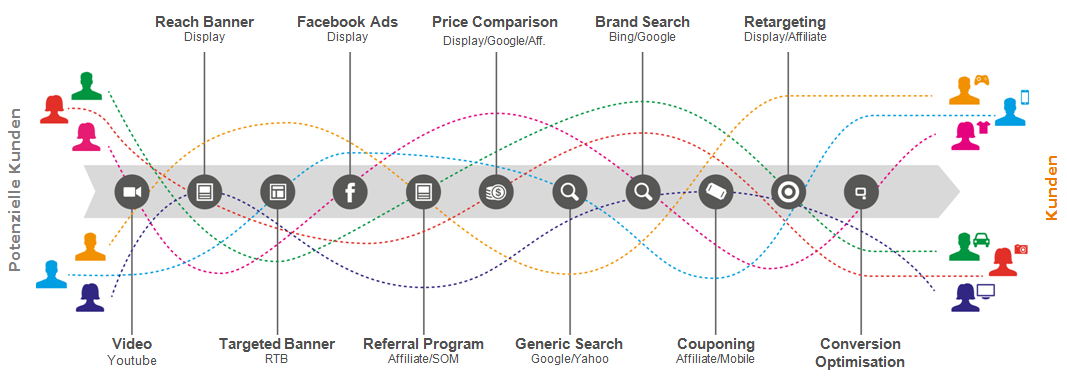
\includegraphics[scale=0.5]{customerJourney.png}\caption[Entstehung eines Funnels]{Entstehung eines Funnels (Quelle: Interhyp AG)}\label{customerJourney}
\end{figure}
\noindent Die Refined Labs GmbH ist auf dem Gebiet des Online-Marketing spezialisiert und verantwortlich für das Online-Tracking der Werbekampagnen der Interhyp AG. Ein Funnel beginnt mit dem ersten Online-Werbekontakt eines potentiellen Kunden mit der Interhyp AG und der damit einhergehenden Erstellung eines Cookies. So können alle weiteren Werbekontakte dem potentiellen Kunden eindeutig zugewiesen werden. Das Tracking endet sobald der potentielle Kunde einen Onlineantrag versendet und damit zum Kunden wird. In diesem Fall spricht man von einem konvertierten Funnel. Wird innerhalb von $90$ Tagen kein Onlineantrag versendet, so wird das Cookie nicht weiter verfolgt und der Funnel wird als nicht-konvertiert bezeichnet.\\
Primäres Ziel dieses Projektes ist das Entdecken von Unterschieden zwischen konvertierten und nicht-konvertierten Funnels. Um dieser Fragestellung gerecht zu werden, wurde ein zeitdiskretes Survival-Modell mittels Stochastic Gradient Boosting geschätzt und ein Sequential Pattern Mining-Algorithmus angewendet. Außerdem wurden die Funnels anhand eines Netzwerkes visualisiert.\\
Die Arbeit ist wie folgt gegliedert. In Kapitel \ref{datenlage} und \ref{descriptiv} werden die Datenaufbereitung und die Variablen erklärt. Daraufhin wird die Methodik des Survival-Modells in Kapitel \ref{survival}, der Sequential Pattern Mining-Algorithmus in Kapitel \ref{spm} und das Netzwerk in Kapitel \ref{network} erläutert. Die Ergebnisse dieser Methoden werden in Kapitel \ref{ergebnisse} vorgestellt und abschließend erfolgt eine Zusammenfassung in Kapitel \ref{zusammenfassung} und die Beschreibung des elektronischen Anhangs in Kapitel \ref{anhang}.
\section{Deskriptive  Analyse}\label{descriptiv}

Tabelle \ref{varbeschreibung} enthält eine Übersicht mit den erzeugten Variablen. Diese werden in diesem Kapitel näher betrachtet. Als Position wird im folgenden die Nummer eines Kontaktpunktes innerhalb eines Funnels bezeichnet. Das heißt für jeden Funnel nimmt der erste Kontakt die Position $1$ an. Die Abbildungen wurden mit dem \textit{R}-Paket \textit{ggplot2} \cite{ggplot2} erzeugt.
\begin{table}[H]
    \begin{center}
\begin{tabular}{|c|p{10cm}|}
		\hline $ clickCount \in \mathbb{N} $ & Anzahl an \textit{Clicks} bis zur aktuellen Position\\
    \hline $ hasClicked\in\{0,1\} $  & Dummyvariable, die angibt ob vor der aktuellen Position schon geklicked wurde ($1$) oder nicht ($0$). \\
		\hline $ campaign $ & Kampagne der aktuellen Position\\ 
    \hline $ campaignLast $ & Kampagne der vorherigen Position\\ 
    \hline $ campaignLast2 $  & Kampagne der vorletzten Position\\
    \hline $ weekday \in \{Montag,...\}$ & Wochentag des Kontaktes  \\
    \hline $ hour \in \{0,1,\dots, 23\} $  & Uhrzeit des Kontaktes \\
    \hline $ timeSinceLast \in \mathbb{R}$  & Zeitdifferenz zwischen aktueller und vorheriger Position\\
    \hline $ timeSinceFirst \in \mathbb{R} $ & Zeitdifferenz zwischen aktueller und erster Position\\
    \hline$ freq \in \mathbb{R} $ & Frequenz der Kontaktpunkte in einem Funnel\\
    \hline
\end{tabular} 
 \end{center}
 \caption{Variablenbeschreibung}\label{varbeschreibung}
\end{table}

\subsection{Views in den konvertierten Funnels}\label{plotsViews}

\subsubsection*{clickCount}
Aufgrund der in Kapitel \ref{datenlage} beschriebenen Problematik bei der Datenerhebung der \textit{Views} können die Variablen \textit{clickCount} und \textit{hasClicked} nur in den konvertierten Funnels betrachtet werden.
\begin{figure}[H]
    \centering
    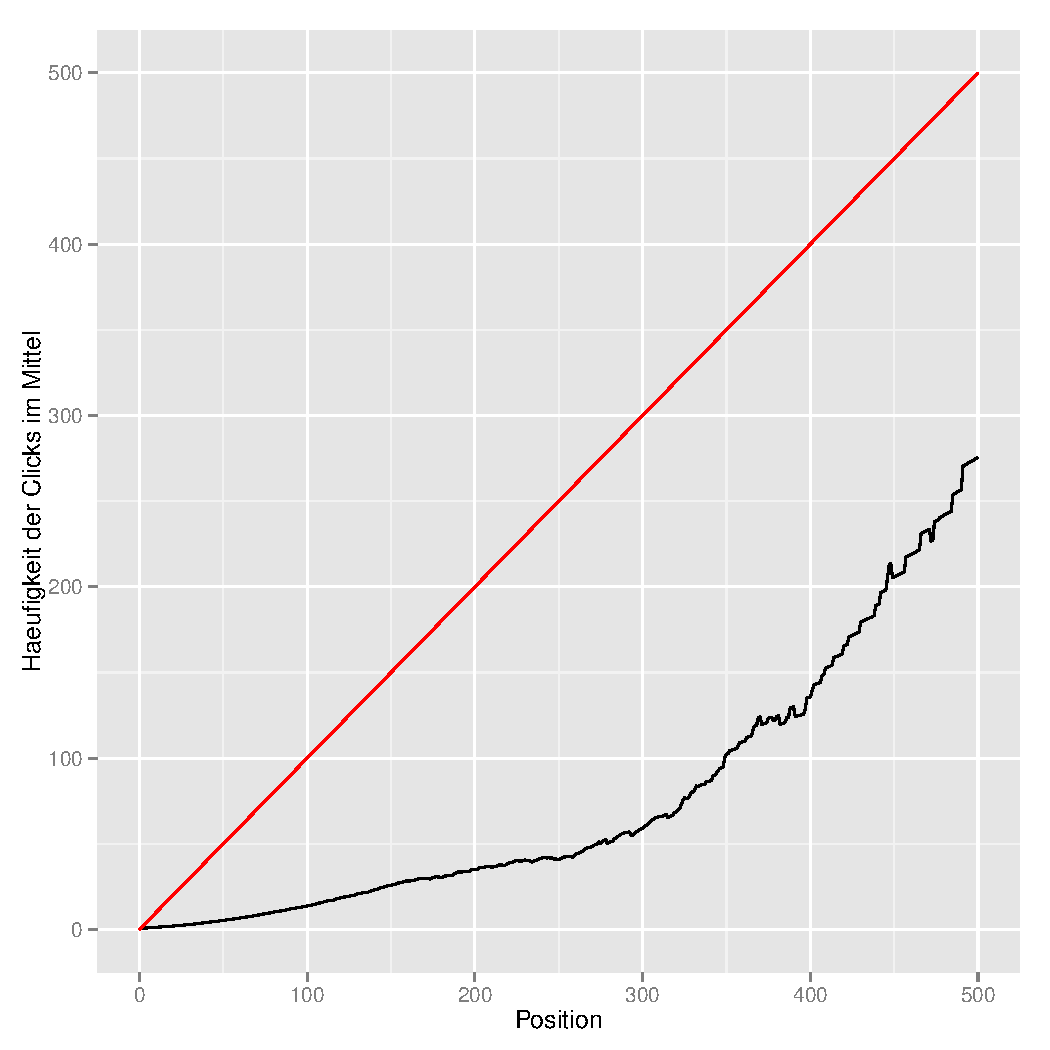
\includegraphics[scale=0.5]{clickCountSucc.pdf}
    \caption[Häufigkeit der Clicks im Mittel]{Häufigkeit der Clicks im Mittel für jede Position}
    \label{clickCount}
\end{figure}
\noindent In Abbildung \ref{clickCount} ist der \textit{clickCount} dargestellt. Auf der $x$-Achse ist die Position aufgetragen und auf der $y$-Achse der \textit{clickCount}, das heißt die Häufigkeit der \textit{Clicks} gemittelt über alle konvertierten Funnels für jede Position. Die rote Diagonale wäre erreicht, wenn die konvertierten Funnels nur aus \textit{Clicks} bestehen würden. Es ist zu erkennen, dass die Linie mit der Position ansteigt. An Position $100$ ist die mittlere Anzahl der Clicks 13.7, das heißt im Mittel bestehen die ersten $100$ Kontakte eines Funnels aus $14$ \textit{Clicks} und $86$ \textit{Views}. Die Anzahl der \textit{Views} übersteigt die Anzahl der \textit{Clicks} also deutlich.\\

\subsubsection*{hasClicked}
Die Variable \textit{hasClicked} (siehe Abbildung \ref{hasClicked}) gibt für jede Position den Anteil der Funnels an, die bis dorthin mindestens einen \textit{Click} enthalten. Dieser Wert nimmt zwischen Position $1$ und Position $7$ ab. Dies ist dadurch zu erklären, dass es viele Funnels gibt, die \textit{Clicks} enthalten und deren Länge kleiner als $6$ ist. Sobald diese Funnels beendet sind, werden sie an der nächsten Position selbstverständlich nicht mehr berücksichtigt. Ab Position $7$ steigt die Kurve dann bis zur $1$ an. Ein Wert von $1$ bedeutet, dass alle Funnels bereits einen \textit{Click} hatten.
\begin{figure}[H]
    \centering
    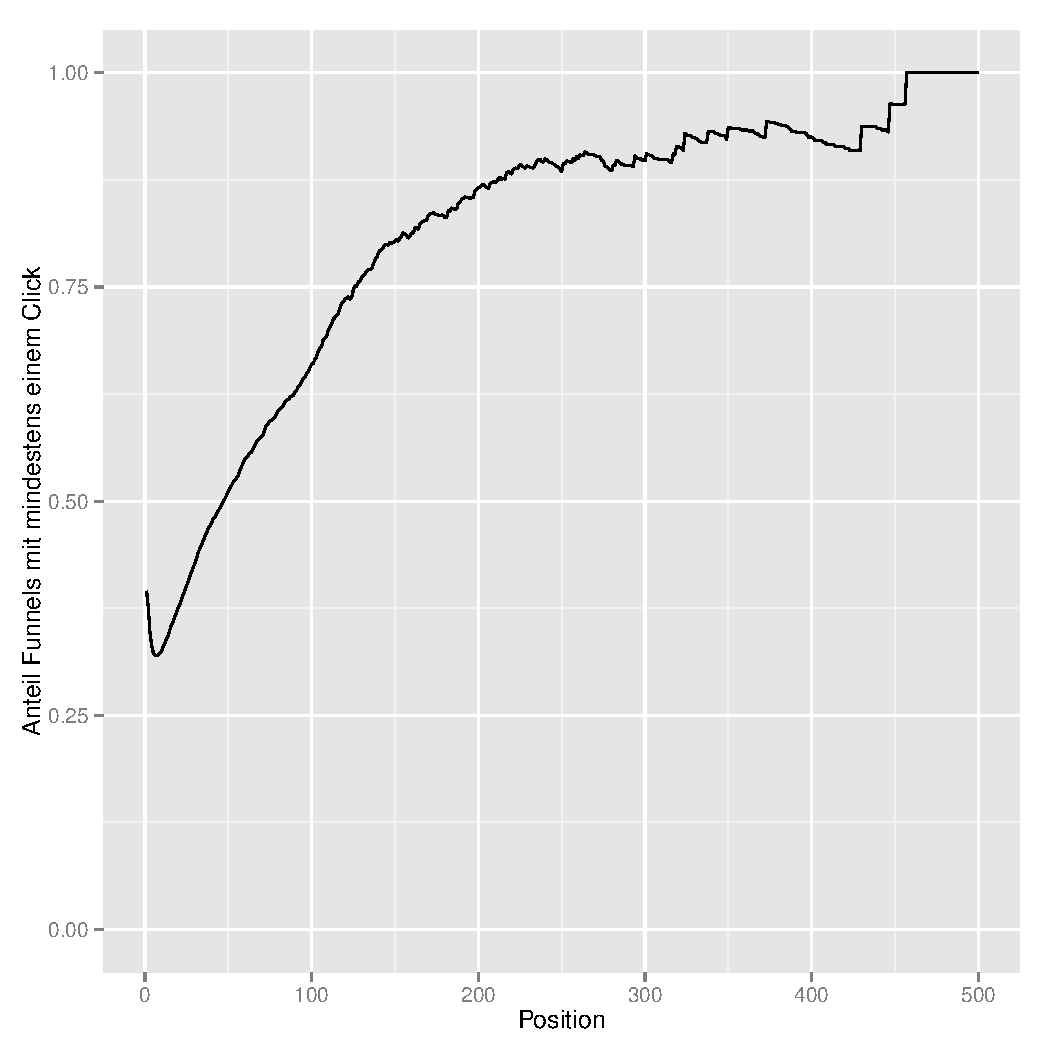
\includegraphics[scale=0.5]{hasClickedSucc.pdf}
    \caption[Anteil Funnels mit mindestens einem Click]{Anteil der Funnels mit mindestems einem Click für jede Position}
    \label{hasClicked}
\end{figure}

\subsubsection*{campaign}
In Kapitel \ref{datenlage} wurde bereits eine Übersicht über die Kampagnen gegeben. Abbildung \ref{campaignSucc} enthält die Verteilung dieser $17$ Kategorien in den konvertierten Funnels, das heißt auf der $x$-Achse ist die relative Häufigkeit aufgetragen und auf der $y$-Achse die Kategorien. Die orangefarbigen Balken repräsentieren die Verteilung in den konvertierten Funnels nur mit \textit{Clicks}, wie sie auch in den späteren Analysen verwendet werden. Die blauen Balken enthalten \textit{Clicks} und \textit{Views}.\\
Es ist zu erkennen, dass die Kampagne \textit{Display} bei den Funnels mit \textit{Views} $84 \%$ der gesamten Kontaktpunkte ausmacht. Das heißt die Bannerschaltungen überwiegen deutlich und ansonsten hat nur \textit{Direct} einen Anteil von über $5 \%$.\\
Werden die \textit{Views} nicht berücksichtigt so verteilen sich die Kampagnen besser. \textit{Display} macht jetzt weniger als $10 \%$ aus und \textit{Direct} ist mit über $35 \%$ die am häufigsten auftretende Kampagne. Außerdem haben auch \textit{SEO}, \textit{SEM - Generisch}, \textit{SEM - Brand}, \textit{Kooperationen - Immoscout24} und \textit{Affiliate - Partnerprogramm} einen Anteil von über $5 \%$. Die restlichen Kampagnen, besonders \textit{Social Media}, machen nur einen kleinen Teil der Daten aus.
\begin{figure}[H]
    \centering
    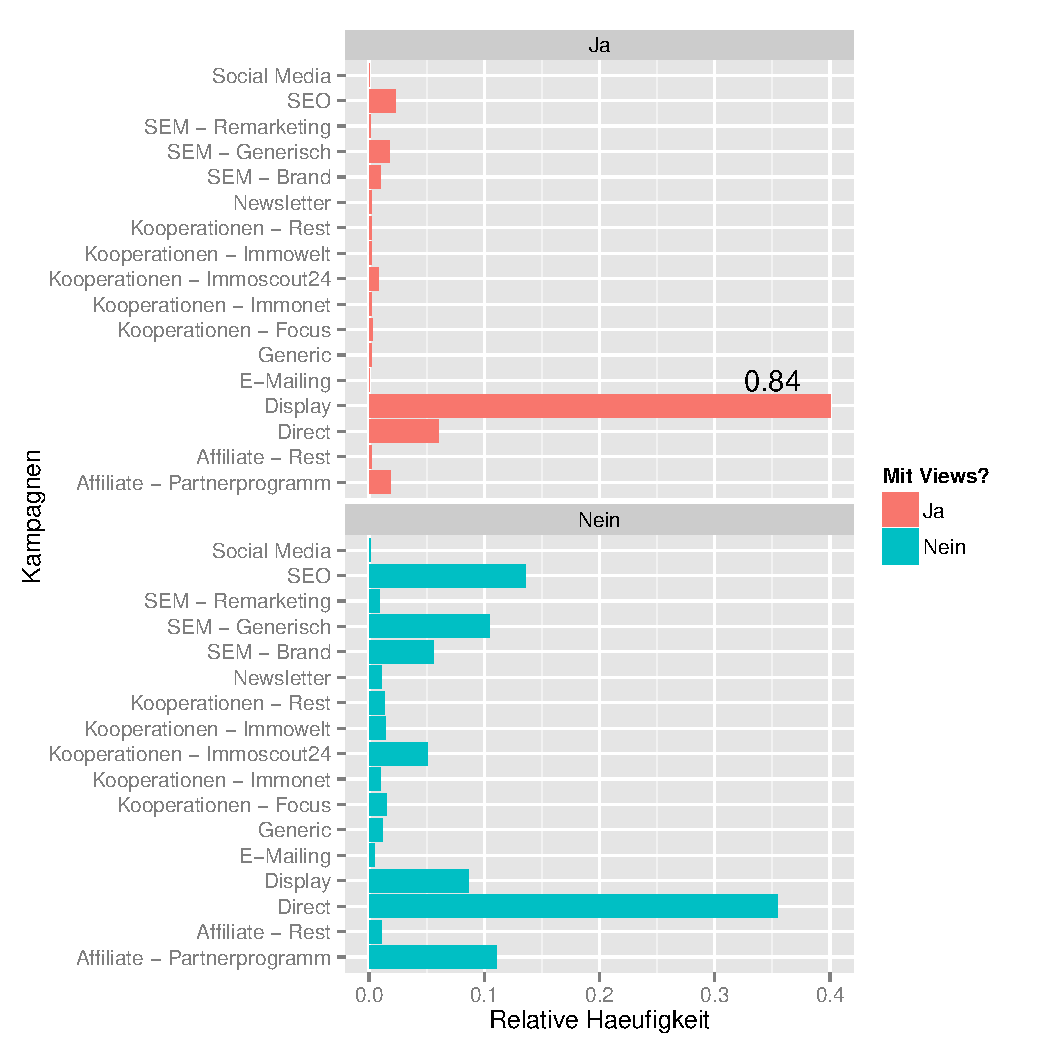
\includegraphics[scale=0.6]{campaignSucc.pdf}
    \caption[Kampagnen der konvertierten Funnels]{Kampagnen der konvertierten Funnels mit und ohne Views}
    \label{campaignSucc}
\end{figure}

\subsection{Vergleich von konvertierten und nicht-konvertierten Funnels}

Nachdem bis hierhin nur die konvertierten Funnels mit Augenmerk auf den \textit{Views} betrachtet wurden, sollen in diesem Kapitel die konvertierten und nicht-konvertierten Funnels miteinander verglichen werden. Das heißt, die \textit{Views} werden von nun an nicht mehr in die Analysen mit einbezogen.

\subsubsection*{weekday}
Die Variable \textit{Weekday} gibt an, an welchem Wochentag ein Konaktpunkt aufgetreten ist. Abbildung \ref{weekday} enthält diesbezüglich Histogramme. Die orangefarbigen Balken entsprechen den konvertierten und die blauen Balken den nicht-konvertierten Funnels. Für weitere Plots in diesem Kapitel gelten die selben Farben. Außerdem ergeben die blauen und orangefarbigen Balken erneut aufsummiert jeweils eins, das heißt sie spiegeln die Verteilung wieder.\\
Es ist zu erkennen, dass die Häufigkeit der Kontaktpunkte von Montag bis Samstag sinkt. Dieser Trend ist in den konvertierten Funnels etwas stärker. Dort sinkt die relative Häufigkeit von $ 0.17 $ am Montag auf $ 0.09 $ am Samstag. Bei den nicht-konvertierten Funnels sinkt die relative Häufigkeit von $ 0.15 $ am Montag auf $ 0.11 $ am Samstag. Außerdem ist der Sonntag bei den nicht-konvertierten mit Abstand der stärkste Tag, während in den konvertierten Funnels der Montag etwas stärker ist als der Sonntag.
\begin{figure}[H]
    \centering
    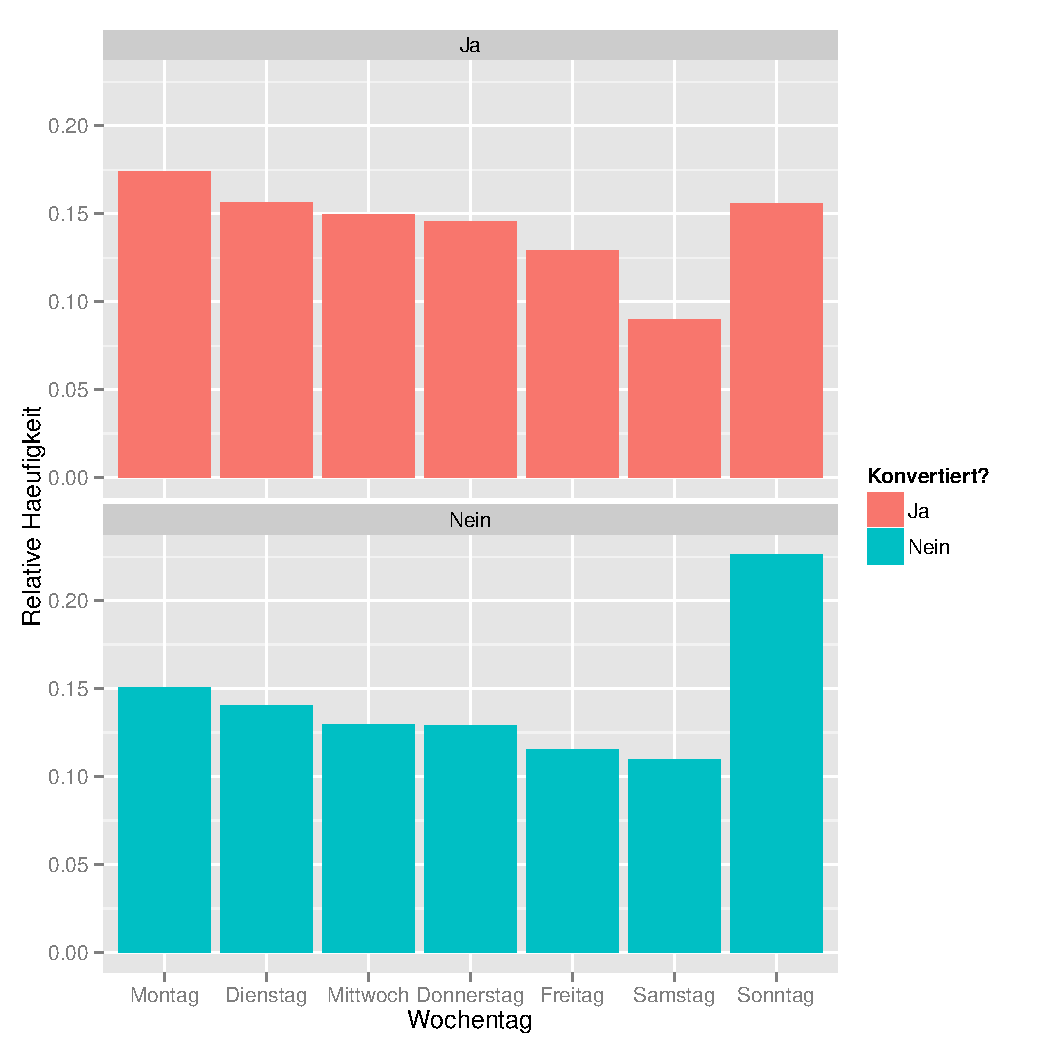
\includegraphics[scale=0.6]{weekday.pdf}
    \caption{Wochentage der Kontaktpunkte}
    \label{weekday}
\end{figure}

\subsubsection*{hour}
Analog zu der Abbildung mit den Wochentagen, enthält Abbildung \ref{hour} Informationen zu der Uhrzeit der Kontaktpunkte in konvertierten und nicht-konvertierten Funnels. Hierfür wurden die Minutenangaben der Uhrzeit jeweils abgeschnitten, so dass \textit{hour} nur die Werte $0,1,...,23$ annehmen kann.\\
\begin{figure}[H]
    \centering
    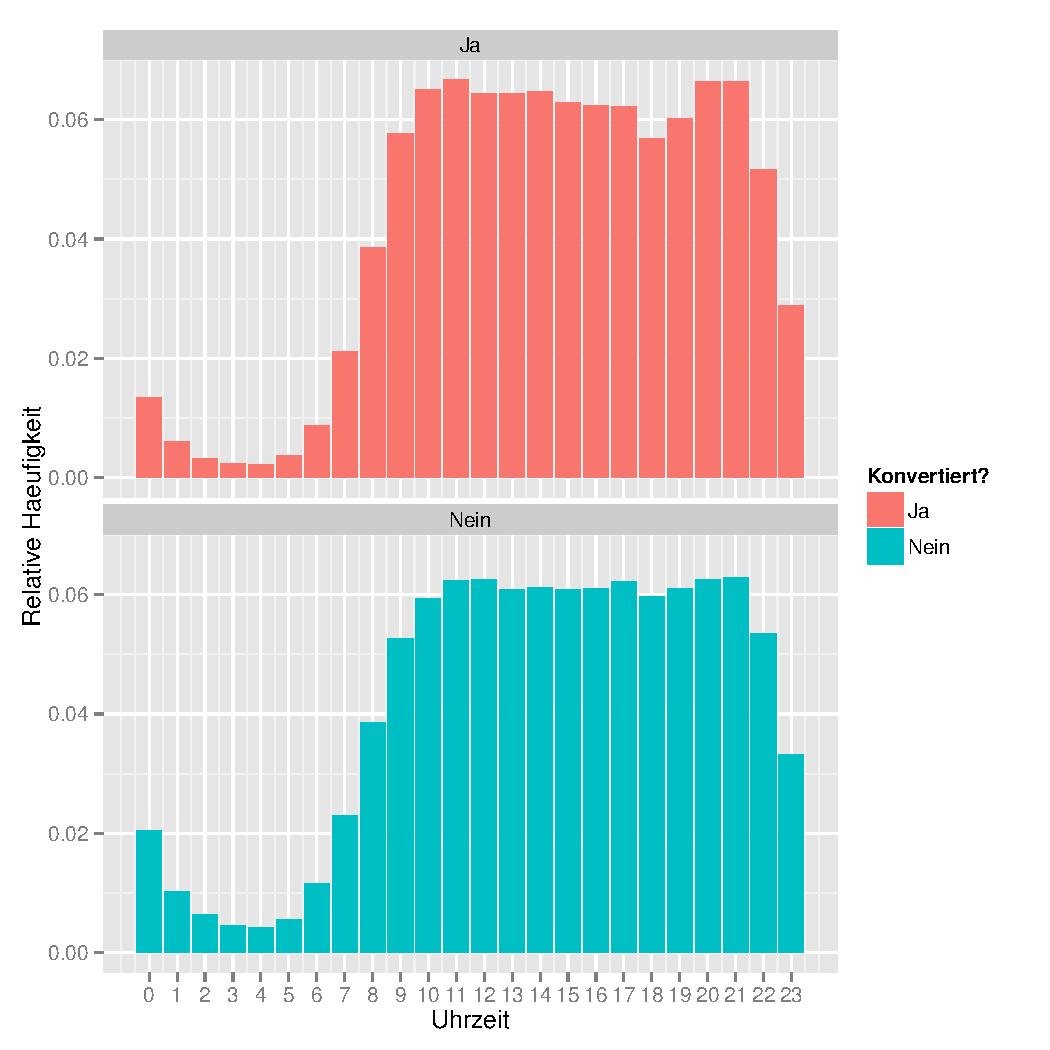
\includegraphics[scale=0.6]{hour.pdf}
    \caption{Uhrzeit der Kontaktpunkte}
    \label{hour}
\end{figure}
\noindent Die Verteilungen in konvertierten und nicht-konvertierten Funnels sind sich sehr ähnlich, so dass keine deutlichen Unterschiede erkennbar sind. Insgesamt kann man zusammenfassen, dass in der Nacht zwischen zwei und sechs Uhr sehr wenige Kontaktpunkte stattfinden. Ab sechs Uhr steigt die relative Häufigkeit der Kontaktpunkte bis circa elf Uhr an und dann bleibt sie konstant bis circa $21$ Uhr. Daraufhin fällt die relative Häufigkeit wieder ab. Dies ist lediglich darauf zurück zu führen, dass nachts weniger Menschen online sind.

\subsubsection*{campaign}
Wie bereits in Kapitel \ref{plotsViews} werden die verschiedenen Kampagnen betrachtet. Allerdings werden an dieser Stelle die konvertierten und nicht-konvertierten Funnels miteinander verglichen, wobei die \textit{Views} nicht berücksichtigt werden (siehe Abbildung \ref{campaign}). Das heißt, die Verteilung der konvertierten Funnels ohne \textit{Views} aus Kapitel \ref{plotsViews} entspricht der Verteilung der konvertierten Funnels in diesem Abschnitt. Eine nähere Beschreibung der unterschiedlichen Kampagnen ist in Abbildung \ref{beschreibungCampaign} zu finden.\\
Die Verteilung in den konvertierten Funnels wurde bereits in Kapitel \ref{plotsViews} etwas näher beleuchtet. Während dort \textit{Direct} mit Abstand die stärkste Kampagne ist, sind in den nicht-konvertierten Funnels \textit{Affiliate - Partnerprogramm} und \textit{Display} die stärksten Kategorien und \textit{Direct} ist lediglich drittstärkste mit einer relativen Häufigkeit von $ 0.123 $. Wie in den konvertierten Funnels haben hier auch \textit{SEO}, \textit{SEM - Generisch} und \textit{Kooperationen - Immoscout24} einen Anteil von über $5 \%$. \textit{SEM - Brand} tritt in den konvertierten Funnels deutlich häufiger auf als in den nicht-konvertierten. Für die restlichen Kampagnen liegen insgesamt wenige Daten vor.

\begin{figure}[H]
	\centering
	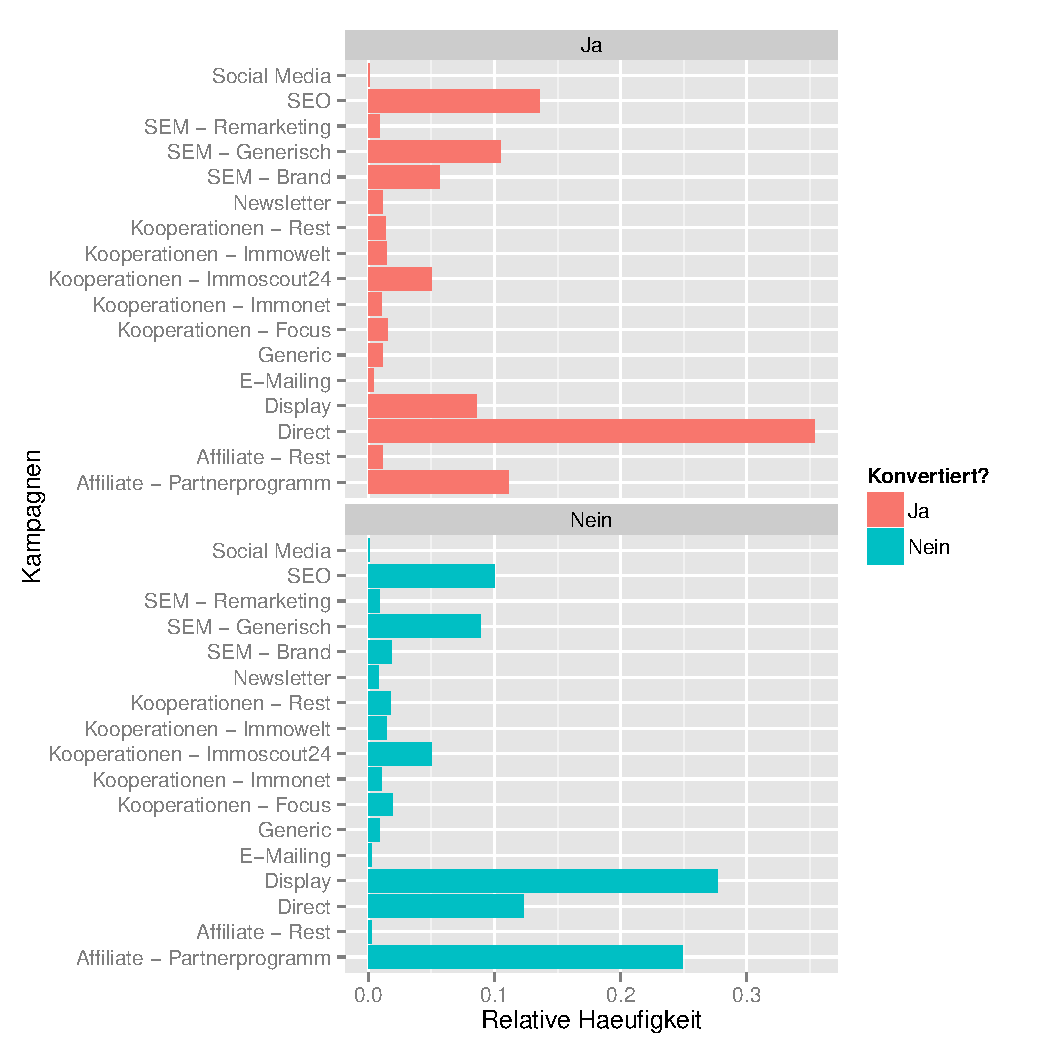
\includegraphics[scale=0.6]{campaign.pdf}
	\caption{Kampagnen der konvertierten und nicht-konvertierten Funnels}
	\label{campaign}
\end{figure}
    
\subsubsection*{funnelLength}
Die \textit{funnelLength} gibt die Anzahl der Kontaktpunkte eines Funnels an. In Abbildung \ref{funnelLength} sind nur diejenigen Funnels dargestellt, deren Länge $20$ Kontaktpunkte nicht überschreitet, da es, relativ gesehen, sehr wenige längere Funnels gibt.\\
Von den nicht-konvertierten Funnels haben $75 \%$ nur einen Kontaktpunkt. Von dort nimmt die relative Häufigkeit der Funnels mit steigender Länge sehr schnell ab. Von den konvertierten Funnels haben $41 \%$ nur einen Kontaktpunkt. Das heißt, relativ betrachtet, gibt es dort mehr Funnels mit mehreren Kontaktpunkten. Allerdings gibt es insgesamt deutlich mehr nicht-konvertierte als konvertierte Funnels, so dass die absoluten Anzahl für die nicht-konvertierten stets größer ist. Der Mittelwert beziehungsweise der Median der Länge der Funnels ist bei den konvertierten Funnels $4.1$ beziehungsweise $2$ und bei den nicht-konvertierten $1.66$ beziehungsweise $1$. 

\begin{figure}[H]
    \centering
    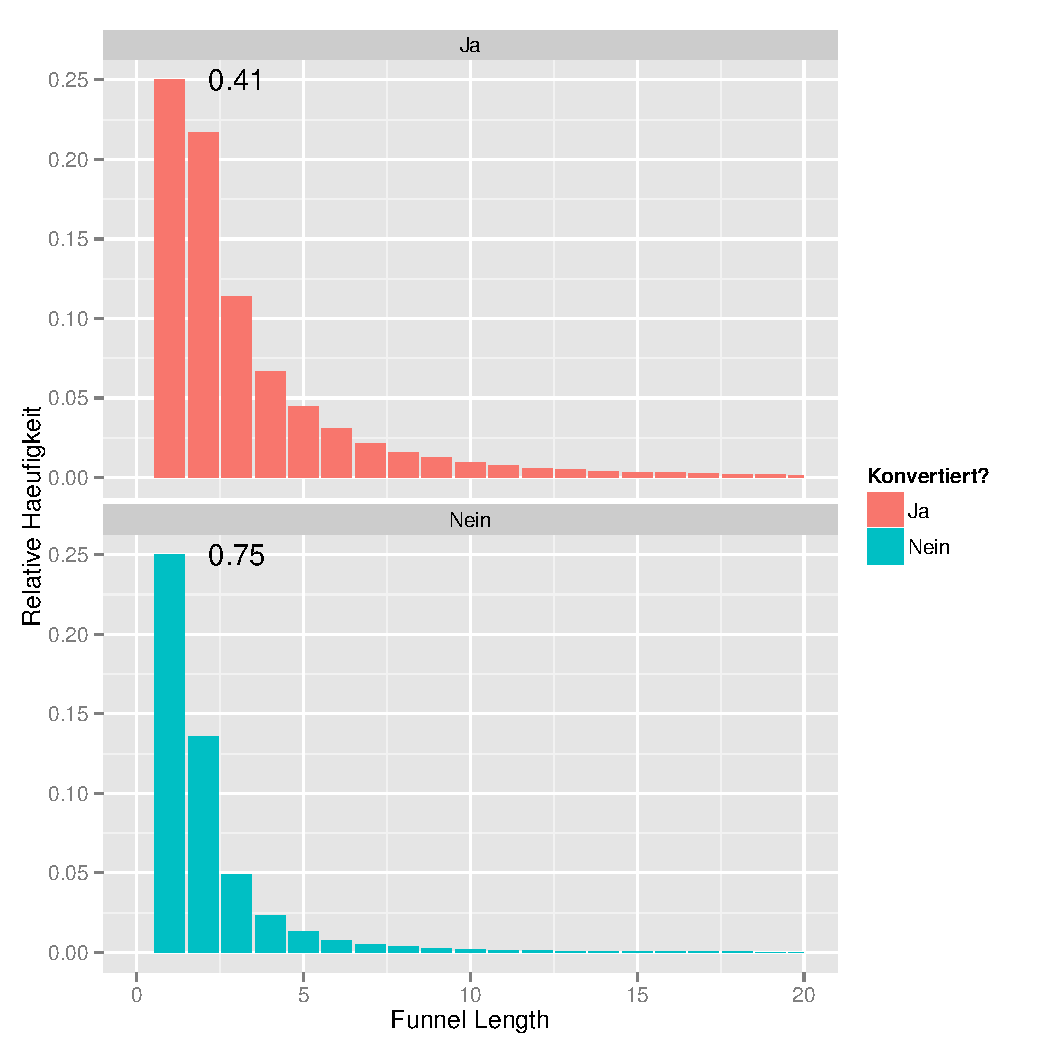
\includegraphics[scale=0.6]{funnelLength_First.pdf}
    \caption[Länge der Funnels]{Länge der Funnels in konvertierten und nicht-konvertierten Funnels}
    \label{funnelLength}
\end{figure}

\subsubsection*{timeSinceFirst}
Das Feature \textit{timeSinceFirst} gibt für jede Position die verstrichene Zeit seit dem ersten Kontaktpunkt an. In Abbildung \ref{timeSinceFirst} wird dieses nur für die letzte Position der Funnels geplottet, so dass die Gesamt-Beobachtungsdauer der Funnels betrachtet wird, das heißt die verstrichene Zeit zwischen dem ersten und dem letzten Kontaktpunkt eines jeden Funnels. Auf der $x$-Achse ist die Beobachtungsdauer in Tagen von $0$ bis $50$ aufgetragen.\\
Hier gestaltet sich ein ähnliches Bild wie in Abbildung \ref{funnelLength}. Allerdings muss berücksichtigt werden, dass die \textit{timeSinceFirst} für die erste Position nicht existiert und somit hier nicht berücksichtigt wird. Von den nicht-konvertierten Funnels haben $58 \%$ eine Beobachtungsdauer von weniger als einem Tag. Längere Beobachtungsdauern treten deutlich seltener auf. Von den konvertierten Funnels haben $33 \%$ eine Beobachtungsdauer von weniger als einem Tag und längere Beobachtungsdauern treten, relativ betrachtet, häufiger auf als in den nicht-konvertierten Funnels.\\
Auffällig sind außerdem die Hückel, die im Rhythmus von sieben Tagen auftreten. Dies ist darauf zurückzuführen, dass Sonntag und Montag die zwei Tage mit den häufigsten Kontakten sind und beispielsweise Bannerschaltungen am Wochenende besonders häufig eingesetzt werden. Bei den konvertierten Funnels liegt der Mittelwert der Beobachtungsdauer bei $21.1$ Tagen und bei den nicht-konvertierten Funnels bei $5.3$ Tagen. 
\begin{figure}[H]
    \centering
    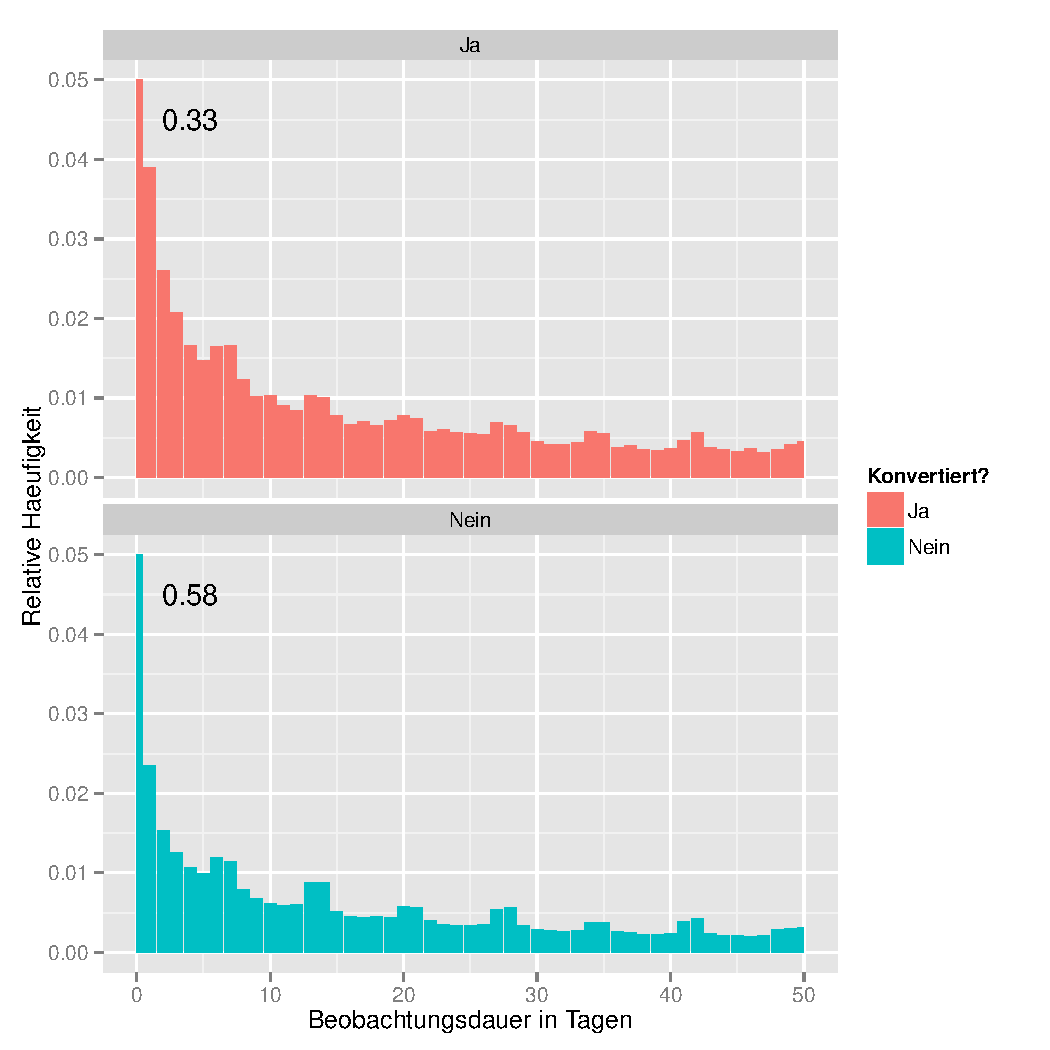
\includegraphics[scale=0.6]{timeSinceFirst_Last.pdf}
    \caption[Beobachtungsdauer in Tagen]{Beobachtungsdauer in Tagen der konvertierten und nicht-konvertierten Funnels}
    \label{timeSinceFirst}
\end{figure}

\subsubsection*{timeSinceLast}
Die Variable \textit{timeSinceLast} gibt die verstrichene Zeit zwischen zwei aufeinander folgenden Kontaktpunkte an. Diese ist in Abbildung \ref{timeSinceLast} abgebildet, wobei nun alle Kontaktpunkte berücksichtigt werden und nicht nur der letzte, wie es bei \textit{timeSinceFirst} der Fall war.\\
Die relative Häufigkeit der Abstände, die kürzer als ein Tag sind ist bei den nicht-konvertierten Funnels höher als bei den konvertierten. Ansonsten sind die Werte bei den konvertierten Funnels höher, wobei wieder ein Abfall mit der Zeit und eine wöchentlich Periodizität zu erkennen sind.\\
Da hier nur die Verteilungen jeweils innerhalb der konvertierten und nicht-konvertierten Funnels verglichen werden, ist \textit{timeSinceLast} keine geeignetes Maß zum Vergleich der Frequenzen der Kontaktpunkte. Dafür wurde die Variable \textit{freq} erzeugt, die im nächsten Abschnitt beschrieben wird.
\begin{figure}[H]
    \centering
    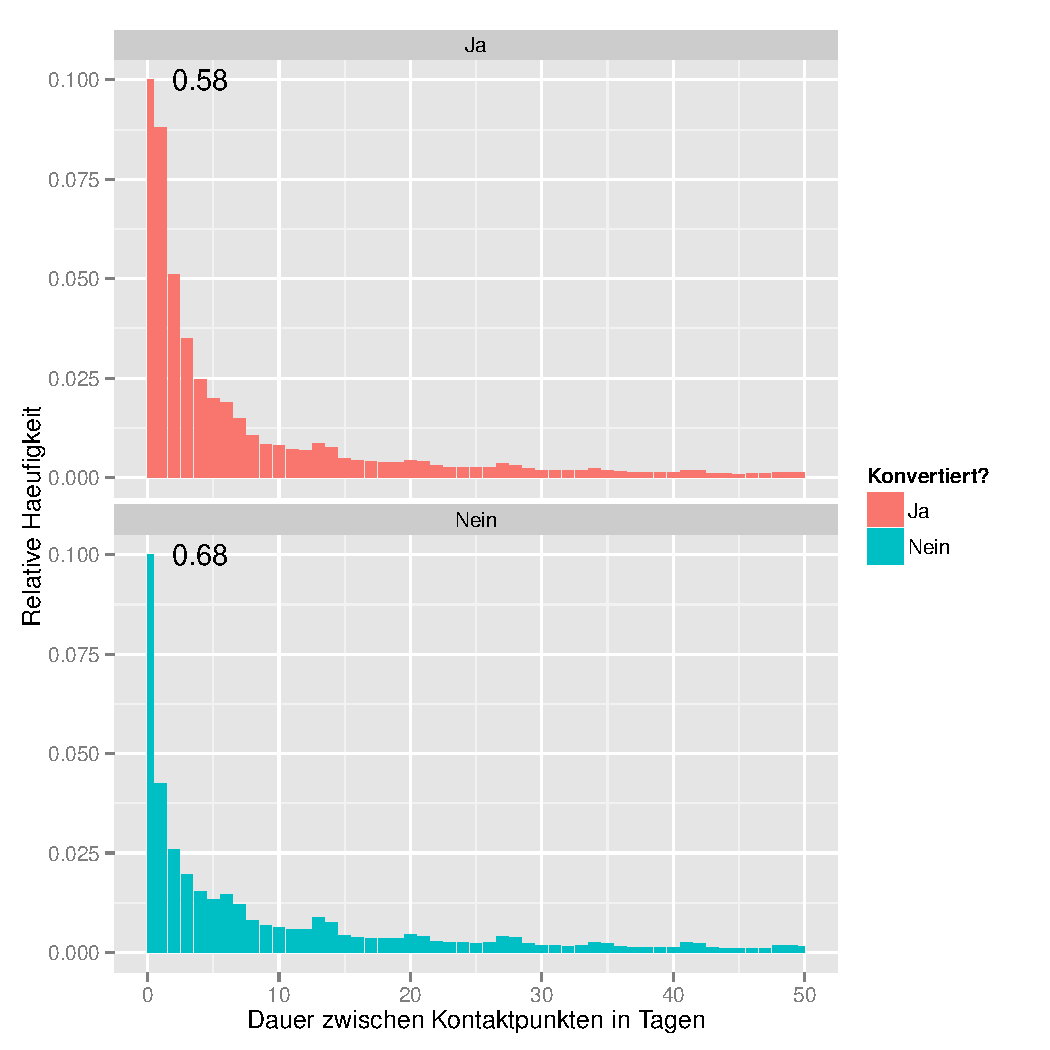
\includegraphics[scale=0.6]{timeSinceLast.pdf}
    \caption[Dauer zwischen zwei Kontaktpunkten]{Dauer zwischen zwei Kontaktpunkten in den konvertierten und nicht-konvertierten Funnels}
    \label{timeSinceLast}
\end{figure}

\subsubsection*{freq}
Die Frequenz wird wie folgt berechnet. Die Daten werden dahingehend gefiltert, dass für jeden Funnel nur der letzte Kontaktpunkt vorhanden ist. Die Variable \textit{timeSinceFirst} gibt somit wieder die Beobachtungsdauer des gesamten Funnels an. Daraufhin wird die Länge des Funnels (siehe Abbildung \ref{funnelLength}) durch die Beobachtungsdauer in Stunden geteilt, so dass eine Größe ensteht, die angibt, wieviel Kontaktpunkte der jeweilige Funnel pro Stunde hatte. Diese Frequenz wird in Abbildung \ref{freq} abgebildet, wobei auf der $x$-Achse die Länge der Funnels zwischen vier und $25$ aufgetragen ist. Für Funnels mit einem Kontaktpunkt existiert offentsichtlich keine Frequenz und die Längen zwei und drei werden nicht mit abgebildet, da die Frequenzen dort verhältnismäßig groß sind. Außerdem sind einige Boxplots nach oben hin abgeschnitten, da die Grenze der $y$-Achse auf $0.15$ gesetzt wurde, damit die Boxplots besser sichtbar sind, wobei der Median, das heißt der schwarze Balken in den Boxplots, für jeden Boxplot erkennbar bleibt. Die orangefarbigen Boxplots entsprechen den Frequenzen der konvertierten und die blauen den Frequenzen der nicht-konvertierten Funnels.\\
Für die Funnel Länge zwei liegt der Median der Frequenzen bei 1.22 in den konvertierten und bei 19.89 in den nicht-konvertierten Funnels sowie für die Länge drei bei 0.021 beziehungsweise 0.348.\\
Insgesamt ist zu erkennen, dass die Frequenzen in den nicht-konvertierten Funnels höher zu sein scheint. Das heißt in denjenigen Funnels die zu keiner Konvertierung führen liegen die Kontaktpunkte näher beieinander, während sie in den konvertierten Funnels mehr über die Zeit verteilt sind.\\
\begin{figure}[H]
		\centering
	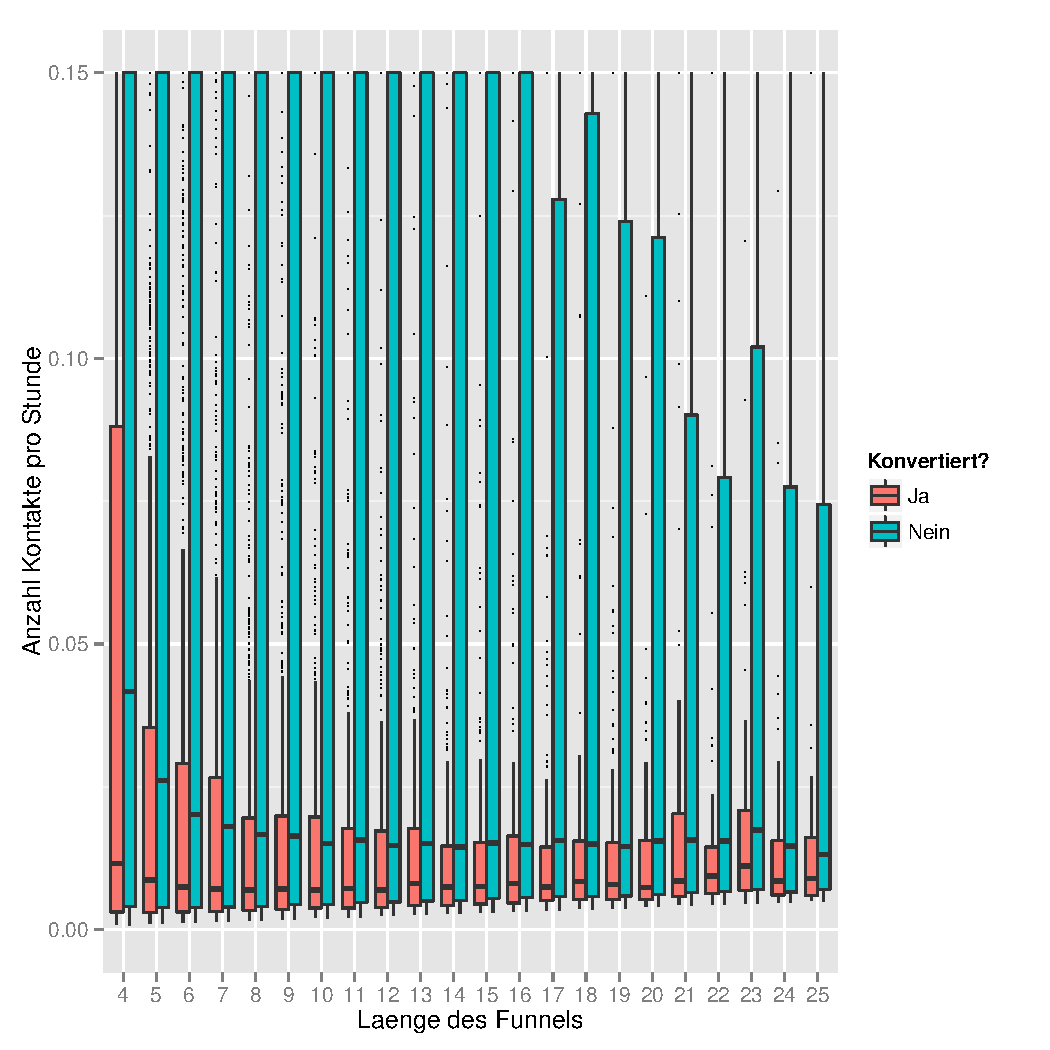
\includegraphics[scale=0.6]{freq.pdf}
	\caption[Frequenz der Kontaktpunkte]{Frequenz der Kontaktpunkte in konvertierten und nicht-konvertierten Funnels}
	\label{freq}
\end{figure}

\section{Methoden}

\begin{frame}\frametitle{Inhalt}
	\tableofcontents[currentsection,hideallsubsections]
\end{frame}

\subsection{Zeitdiskretes Survival-Modell}

\begin{frame}
	\begin{itemize}
		\item Zeit bis zu einem Ereignis $\Rightarrow$ Konvertierung oder Nicht-Konvertierung bzw. Rechtszensierung
		\item Positionen bilden Zeitachse des Modells $\Rightarrow$ Zeitdiskretes Modell
		\item Stochastic Gradient Boosting mit Stümpfen als Basis-Lerner
	\end{itemize}
\end{frame}

\begin{frame}
	\begin{itemize}
		\item Zielvariable:	
			\begin{align*}
				y_{ip} =& \begin{cases} 1 & \text{Beobachtung } i \text{ konvertiert an Position } p\\
															 0 & \text{sonst} 
								 \end{cases}\\
								&p=1,...,25 \text{, } i=1,...,N_p 
			\end{align*}	
		\item Hazardrate: 
			\begin{align*}
				\lambda_{ip} = P(y_{ip}=1|funnelLength_i \geq p, x_{ip})
			\end{align*}
		\item Logit-Modell: 
			\begin{align*}
				y_{ip}|x_{ip} &\stackrel{ind}{\sim} Bin(1, \lambda_{ip})  \\
				E(y_{ip}|x_{ip}) = P(y_{ip} = 1|x_{ip}) = \lambda_{ip} &= h(f_{ip}) = \frac{\exp(f_{ip})}{1+\exp(f_{ip})}
			\end{align*}
	\end{itemize}
\end{frame}

\begin{frame}
	\begin{itemize}
		\item Likelihood: 
			\begin{align*}
				L(\lambda_{ip}) &= \prod_{i=1}^{N_p} \lambda_{ip}^{y_{ip}} (1-\lambda_{ip})^{1-y_{ip}}
			\end{align*}
		\item Log-Likelihood: 
			\begin{align*}
				l(\lambda_{ip}) &= \ln(L(\lambda_{ip})) = \sum_{i=1}^{N_p} (y_{ip} \ln(\lambda_{ip}) + (1-y_{ip}) \ln(1-\lambda_{ip}))\\
				&= \sum_{i=1}^{N_p} (y_{ip} f(x_{ip}) - \ln(1+\exp(f(x_{ip}))))
			\end{align*}
		\item Binomieller Verlust: 
			\begin{align*}
				L(y,f) = -yf + \ln(1+\exp(f))
			\end{align*}
	\end{itemize}
\end{frame}

\begin{frame}
	\begin{itemize}
		\item Prädiktorfunktion:
			\begin{align*}
			f(x_{ip}) =&f_{weekday,p}(\text{weekday}_{ip}) +\\
								 &f_{hour,p}(\text{hour}_{ip}) +\\
								 &f_{campaign,p}(\text{campaign}_{ip}) +\\
								 &f_{campaignLast,p}(\text{campaign}_{i,p-1}) +\\
								 &f_{campaignLast2,p}(\text{campaign}_{i,p-2}) +\\
								 &f_{timeSinceLast,p}(\text{timeSinceLast}_{ip}) +\\
								 &f_{timeSinceFirst,p}(\text{timeSinceFirst}_{ip}) +\\
								 &\text{offset}(\hat{\lambda}_{i,p-1})
			\end{align*}
	\end{itemize}
\end{frame}

\begin{frame}\frametitle{Gradient Boosting - Pseudocode}
	\floatname{algorithm}{Algorithmus}
	%\begin{algorithm}
	%\caption{Gradient Boosting}\label{alg}
	%\label{gradboosting}
		\begin{algorithmic}
		\STATE Setze Startwert für $f_{0p}(x_{ip})$
		\FOR{$m=1:n.trees$}
			\STATE Setze $\lambda_{ip}(x_{ip}) = \frac{\exp(f_{m-1,p}(x_{ip}))}{1+\exp(f_{m-1,p}(x_{ip}))}$
			\FOR{$i=1:N_p$} 
				\STATE $r_{imp} = - \frac{\partial L(y_{ip},f_{m-1,p}(x_{ip}))}{\partial f_{m-1,p}(x_{ip})} = y_{ip} - \lambda_{ip}(x_{ip})$
			\ENDFOR
			%\STATE Fit a regression base learner to the pseudo-residuals $r_{im}$:
			\STATE $\theta_{mp} = \argmin_{\theta} \sum_{i=1}^{N_p} (r_{imp} - h(x_{ip}, \theta))^2$
			\STATE $\beta_{mp} = \argmin_{\beta} \sum_{i=1}^{N_p} L(y_{ip}, f_{m-1,p}(x_{ip}) + \beta h(x_{ip},\theta_{mp}))$
			\STATE $f_{mp}(x_{ip}) = f_{m-1,p}(x_{ip}) + \beta_{mp} h(x_{ip},\theta_{mp})$
		\ENDFOR
		\end{algorithmic}
	%\end{algorithm}
\end{frame}

\begin{frame}\frametitle{Parameter des Modells}
	\begin{itemize}
		\item Trainingsdaten machen Hälfte der gesamten Daten aus - stratifiziert bezüglich Transaction, Campaign, funnelLength
		\item $n.trees=3000$
		\item $cv.folds=5$
		\item Shrinkage-Parameter: $\mu = 0.01 \Rightarrow f_{mp}(x_{ip}) = f_{m-1,p}(x_{ip}) + \mu \beta_{mp} h(x_{ip},\theta_{mp})$
		\item $interaction.depth=1$
		\item $bag.fraction=0.5 \Rightarrow$ \textbf{Stochastic} Gradient Boosting
	\end{itemize}
\end{frame}

\begin{frame}\frametitle{Output des Modells}
	\begin{itemize}
		\item $\hat{f}(x_{ip})$ für jede Beobachtung $i$ und jede Position $p$
			\begin{align*}
				\hat{\lambda}_{ip} = \frac{\exp(\hat{f}(x_{ip}))}{1+\exp(\hat{f}(x_{ip}))}
			\end{align*}
		\item Relative Wichtigkeit der Features:
			\begin{align*}
				\hat{I}_{jp} &= \sqrt{\frac{1}{M} \sum_{m=1}^{n.trees} \hat{i}_{mp} 1_{jmp}}
			\end{align*}
		\item Marginale Effekte der Features:
			\begin{align*}
				\bar{f}_{jp}(x_{jp}) = \frac{1}{N} \sum_{i=1}^{N_p} \hat{f}(x_{jp},x_{i,\backslash j,p})
			\end{align*}
		\item ROC-Kurve und AUC
	\end{itemize}
\end{frame}

\subsection{Sequential Pattern Mining}

\begin{frame}
	\begin{itemize}
		\item Menge von Items $I = \{a, b, c, d, e\}$ $\Rightarrow$ Kampagnen
		\item Datenbank: $[ID 1, <abcdbaae>]$; $[ID 2, <edcaa>]$
		\item 4-Sequenz $s = b\rightarrow b\rightarrow a\rightarrow e$
		\item Support einer Sequenz: Anteil der IDs, die $s$ unterstützen
		\item SPADE-Algorithmus findet häufige Sequenzen, deren Support größer als ein festgelegter minimaler Support ist
		\item Seperate Anwendung auf konvertierte und nicht-konvertierte Funnels
	\end{itemize}
\end{frame}

\subsection{Visualisierung anhand eines Netzwerkes}

\begin{frame}
	\begin{itemize}
		\item Geordneter Graph $G=(V,E)$ besteht aus Menge $V$ von Knoten und Menge $E$ von Kanten
		\item Kante $e_i \in E$ besteht aus geordneten Paar von zwei Knoten $(v_j,v_k)$, wobei $v_j,v_k \in V$
		\item Startpunkt $\rightarrow$ $17$ Kampagnen der ersten Position $\rightarrow$ $Succ\_1$, $Fail\_1$ und $17$ Kampagnen der zweiten Position $\rightarrow$ $Succ\_2$, $Fail\_2$ und $17$ Kampagnen der dritten Position $\rightarrow$ ...
		\item Kanten sind bezüglich der Anzahl der Nutzer gewichtet
		\item Relative Ausgänge: relative Häufigkeiten der Kanten, wobei die zugrundeliegende Menge die Summe aller Nutzer ist, die einen Knoten verlassen
		\item Relative Eingänge: relative Häufigkeiten der Kanten, wobei die zugrundeliegende Menge die Summe aller Nutzer ist, die in einen Knoten gehen
	\end{itemize}
\end{frame}

\begin{frame}
	\begin{itemize}
		\item \textit{R}-Paket \textit{rgexf} $\rightarrow$ \textit{gexf}-Datei $\rightarrow$ \textit{Gephi}
		\item Berechnung der räumlichen Anordnung der Knoten und Kanten anhand von Algorithmen (z.B. \textit{Force Atlas 2})
		\item Manuelle Bearbeitung für die Präsentation von Ergebnissen
		\item Interaktives Arbeiten mit dem Netzwerk in \textit{Gephi} möglich $\rightarrow$ Tutorial dazu im Bericht
	\end{itemize}
	\centering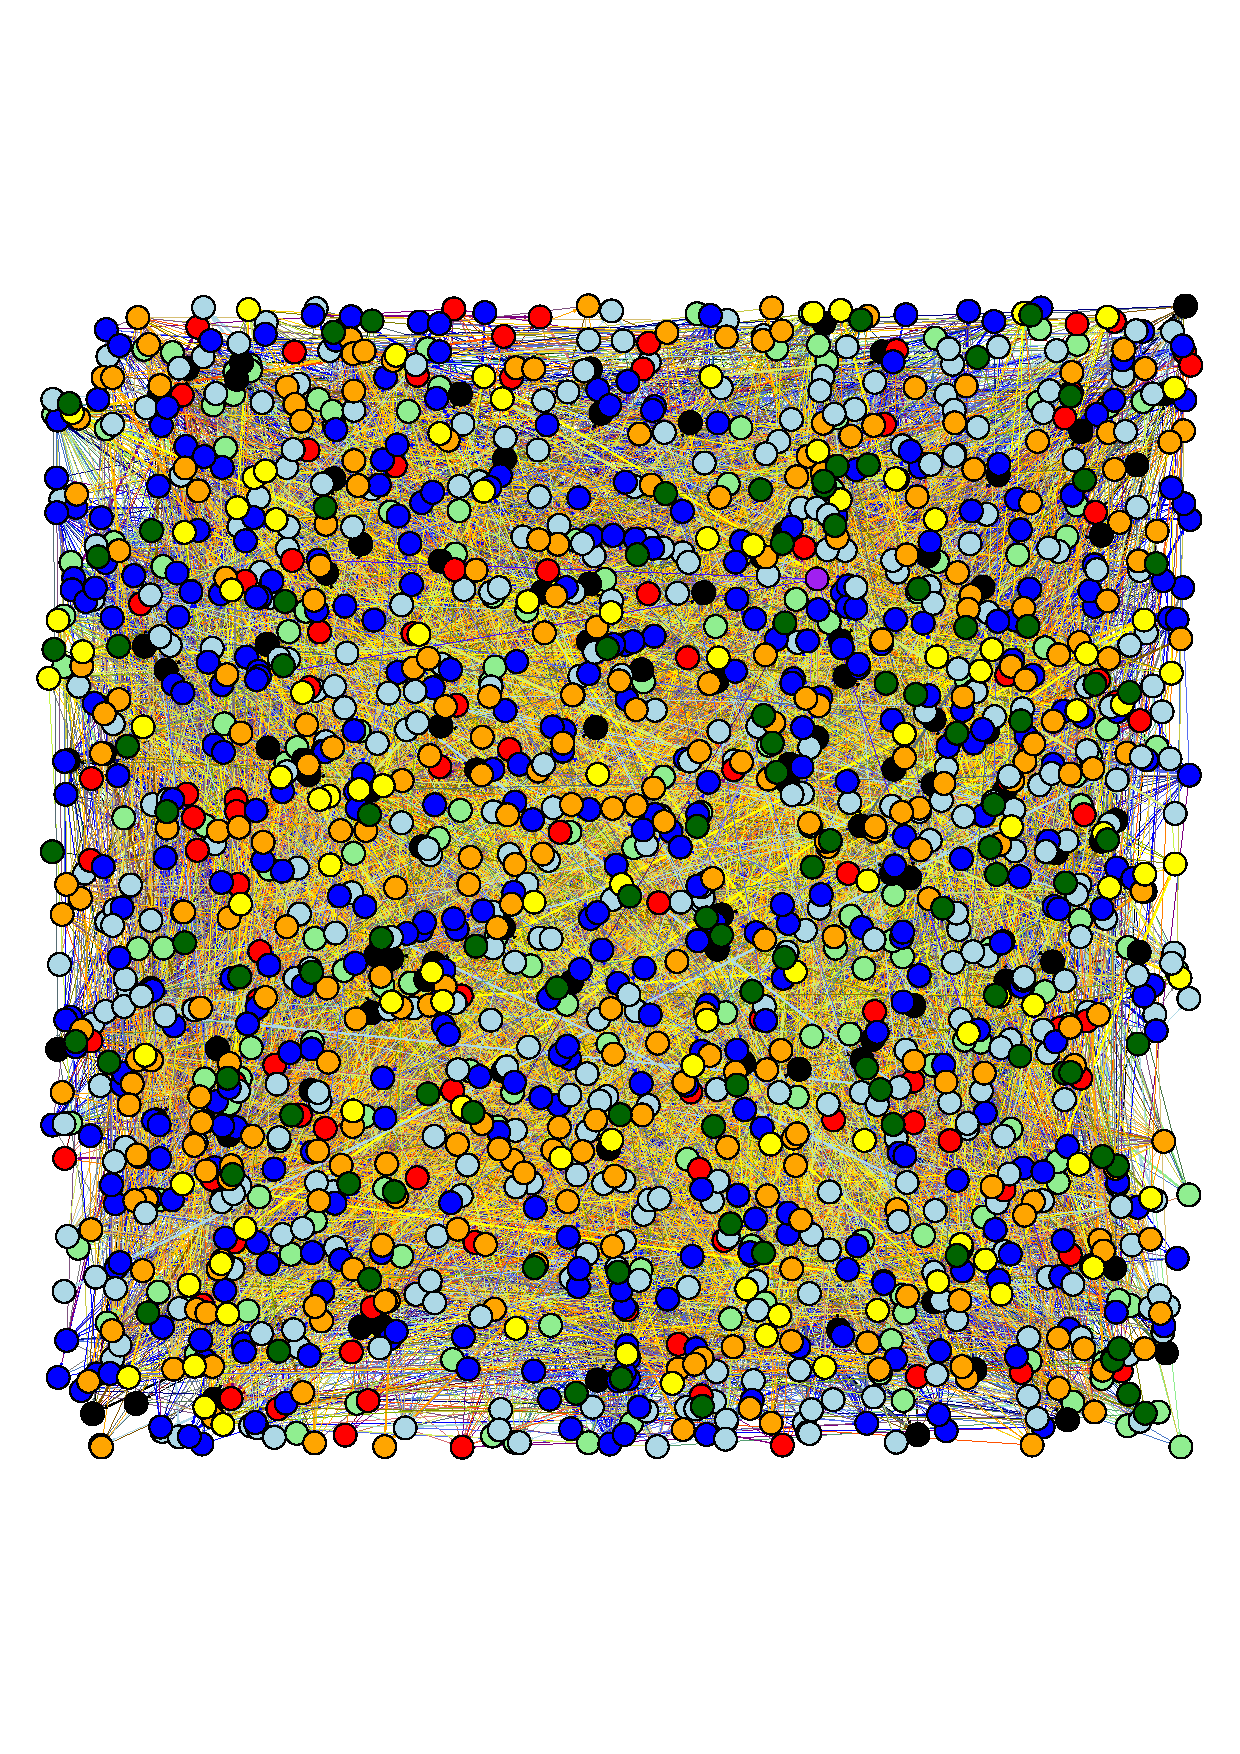
\includegraphics[scale=0.2]{graphbegin.pdf}
\end{frame}

\section{Ergebnisse}\label{ergebnisse}

\subsection{Zeitdiskretes Survival-Modell}

Die in diesem Kapitel präsentierten Ergebnisse basieren jeweils auf der bestmöglichen Anzahl an Iterationen. Diese wurden mittels $5$-facher Kreuzvalidierung ermittelt und sind in Abbildung \ref{best_iter} dargestellt. Auf der $x$-Achse ist die Position von $1$ bis $25$ aufgetragen und auf der $y$-Achse die Optimale Iterationsanzahl, die durch $n.trees = 3000$ nach oben begrenzt ist. Es ist zu erkennen, dass für die Positionen $1$ bis $4$ über $2500$ Stümpfe für die Ergebnisse verwendet werden. Dann fällt die Kurve sehr schnell ab bis sie sich bei ungefähr $500$ Iterationen einpendelt. Dieser Abfall ist dadurch zu erklären, dass mit steigender Position die Datenmenge sinkt.\\
\begin{figure}[H]
	\centering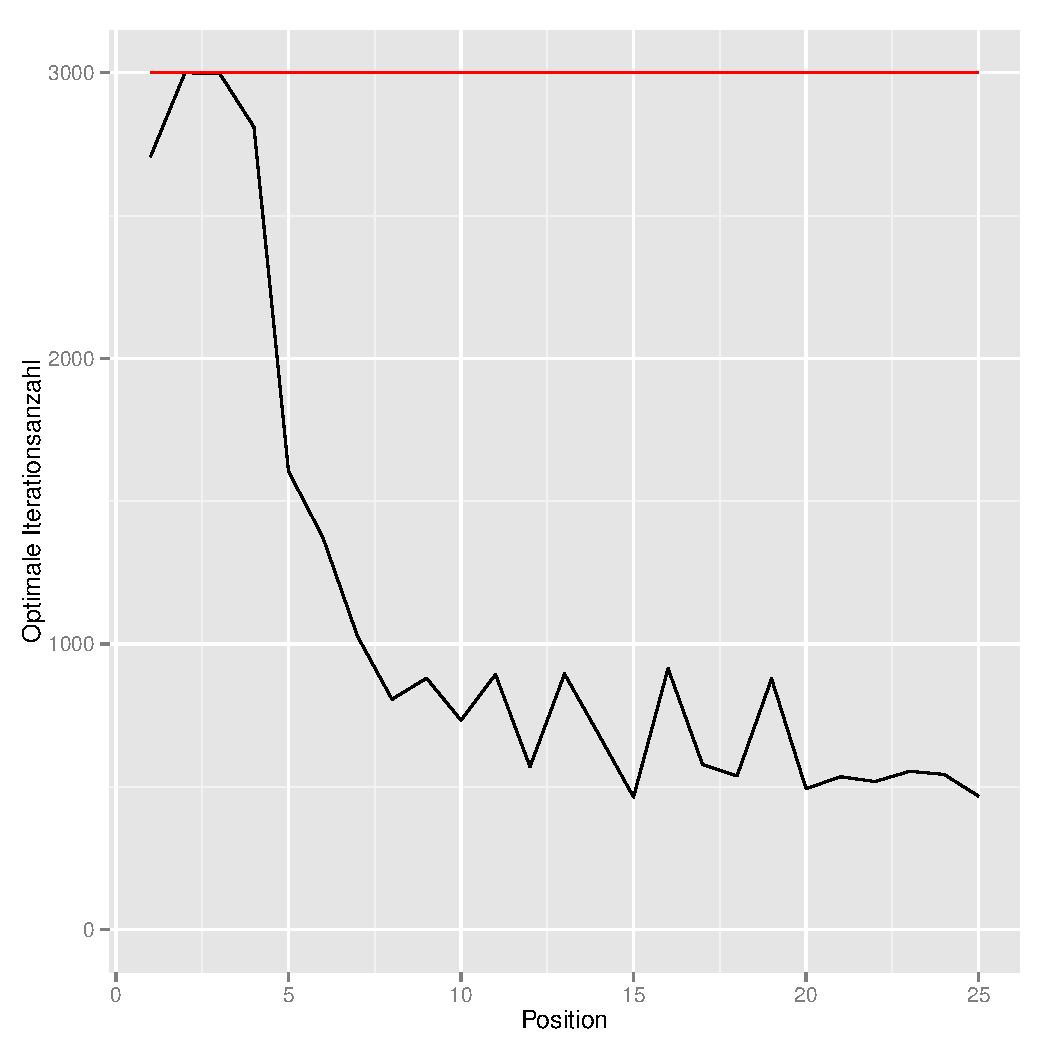
\includegraphics[scale=0.5]{bestIter.pdf}\caption[Optimale Iterationsanzahl]{Optimale Iterationsanzahl des Stochastic Gradient Boosting}\label{best_iter}
\end{figure}
\noindent Der relative Einfluss der Features gibt dessen Wichtigkeit bei der Erstellung der Prädiktorfunktion an und ist in Abbildung \ref{variable_importance} dargestellt. Auf der $x$-Achse ist erneut die Position aufgetragen und auf der $y$-Achse der relative Einfluss. Der relative Einfluss aller Features an einer Position ergibt summiert jeweils $100$ und die Balken sind der Größe nach geordnet, das heißt die wichtigsten Variablen sind unten abgebildet. Die Farben der Balken werden in der Legende rechts neben der Abbildung erläutert.\\
An Position $1$ sind nur drei Features vorhanden, wobei $Campaign$, das heißt die Art des Kontaktpunktes, für circa $90 \%$ der Minimierung der Verlustfunktion verantwortlich ist. Die Variablen $Hour$ und $Weekday$ haben kaum Einfluss. An Position $2$ ist die Kampagne immer noch das stärkste Feature, wobei hier auch die Kampagne des ersten Kontaktpunktes und die Zeit, die seit dem ersten Kontaktpunkt vergangen ist, Einfluss haben.\\
An den Positionen $8$ und $22$ hat die Kampagne des letzten Kontaktpunktes den stärksten Einfluss und damit selbstverständlich auch einen höheren Einfluss als die Kampagne des aktuellen Kontaktpunktes, die insbesondere an den höheren Positionen oft nur noch einen geringen Einfluss hat. Mit steigender Position wird auch die Kampagne des vorletzten Kontaktes wichtiger und ist manchmal das wichtigste Feature. Die Zeit, die seit dem vorherigen Kontaktpunkt vergangen ist, ist bereits an Position $3$ zweitwichtigstes Feature und spielt auch für die folgenden Positionen eine Rolle. Später nimmt die Wichtigkeit dieses Features allerdings ab und die Zeit, die seit dem ersten Kontaktpunkt vergangen ist, wird bedeutend wichtiger. Die Features $Hour$ und $Weekday$ spielen positionsübergreifend kaum eine Rolle.\\
Nachdem die Wichtigkeit der Variablen für die Klassifizierung in konvertierte und nicht-konvertierte Funnel präsentiert wurde, ist nun die Art dieses Einflusses interessant. Dieser wird im folgenden für einige Positionen dargestellt, wobei die Variablen dafür nach positionsspezifischer Wichtigkeit ausgesucht werden und das Augenmerk vor allem auf die niedrigeren Positionen fällt, da dort mehr Daten vorhanden sind. Folglich werden die Features $Hour$ und $Weekday$ garnicht präsentiert, das sie kaum einen Einfluss haben. Die Kampagne des vorletzten Kontaktpunktes $CampaignLast2$ wird an dieser Stelle ebenfalls nicht berücksichtigt, da die Ergebnisse für $Campaign$ beziehungsweise $CampaignLast$ oft sehr ähnlich sind. Im elektronischen Anhang sind die marginalen Effekte aller Features für jeweils jede Position zu finden.
\begin{figure}[H]
	\centering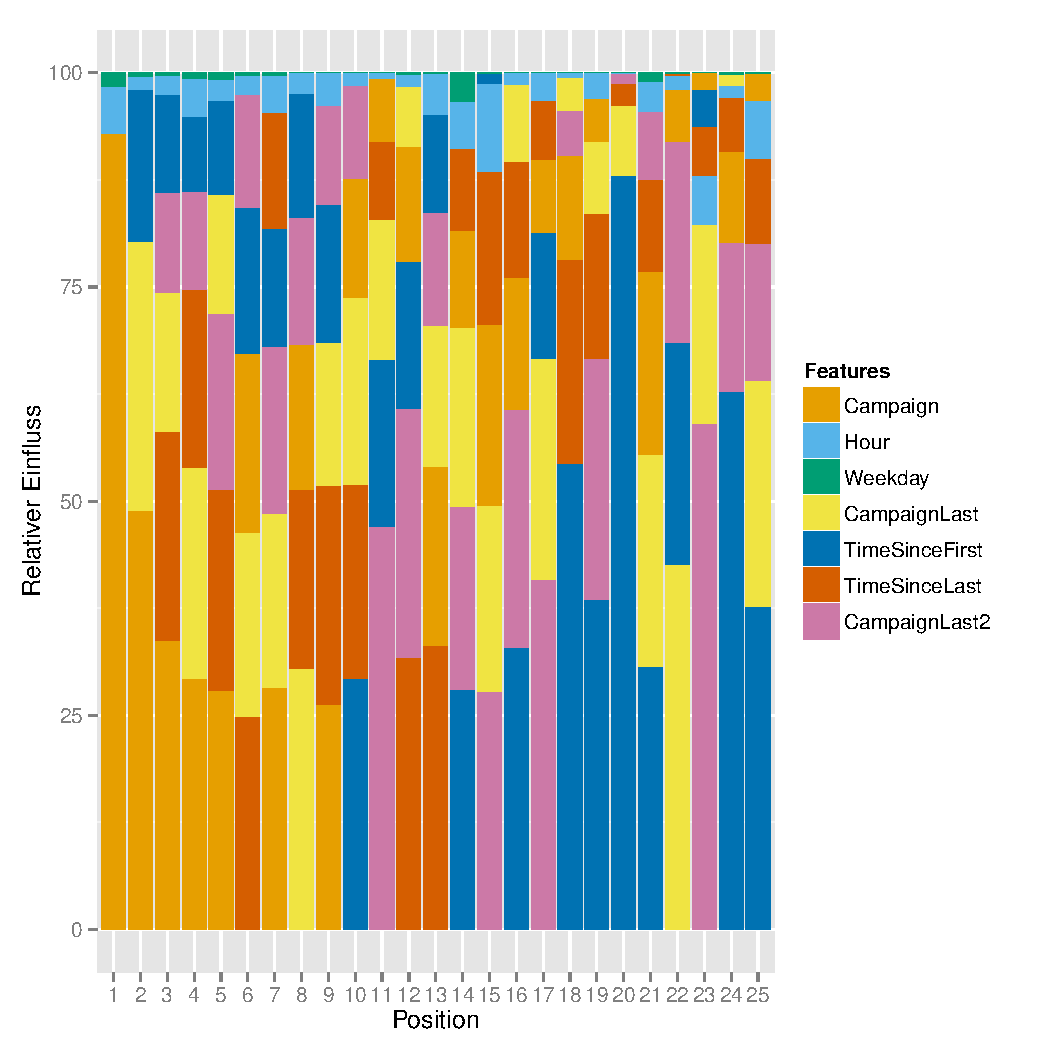
\includegraphics[scale=0.9]{variableImportance.pdf}\caption{Wichtigkeit der Variablen}\label{variable_importance}
\end{figure}
In Abbildung \ref{marg_eff_campaign} sind die marginalen Effekte der Variable \textit{Campaign} für die Positionen eins bis vier, von links oben nach rechts unten, aufgetragen. \textit{Campaign} ist an den ersten vier Positionen das wichtigste Feature. Mit steigender Position verliert die Variable deutlich an Einfluss. Auf der $x$-Achse ist die Art des aktuellen Kontaktpunnktes aufgetragen und auf der $y$-Achse der Marginale Effekt.\\
An Position eins haben die Kampagnen \textit{Affiliate - Rest}, \textit{E-Mailing} und \textit{SEM - Brand} im Vergleich zu den restlichen Kampagnen einen starken, positiven Einfluss auf die Konvertierungswahrscheinlichkeit.
\begin{figure}[H]
	\centering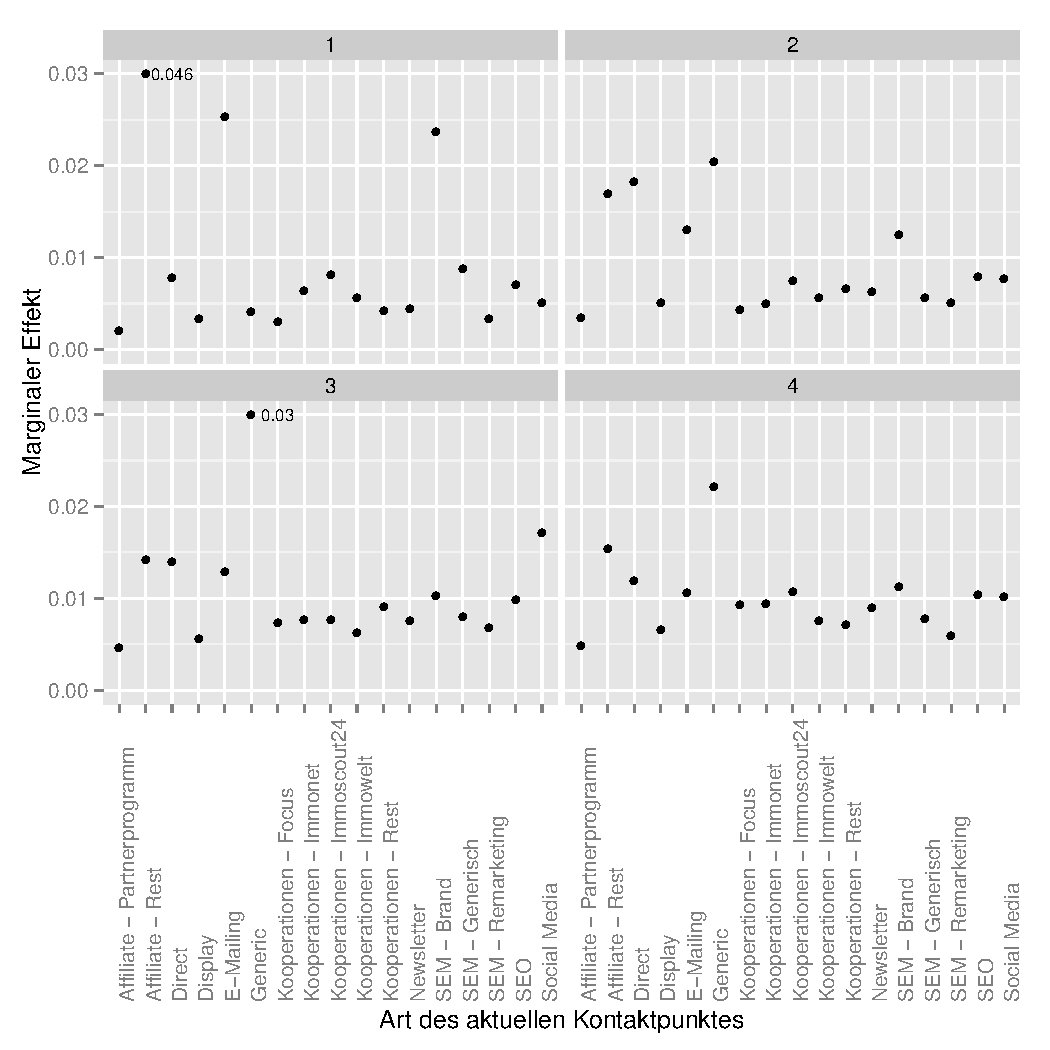
\includegraphics[scale=0.75]{marg_eff_campaign.pdf}\caption[Marginaler Effekt von \textit{Campaign}]{Marginaler Effekt des Features \textit{Campaign} an den Positionen $1$, $2$, $3$ und $4$}\label{marg_eff_campaign}
\end{figure}
\noindent Das heißt das Bereitstellen von Zinsvergleichen, welche das Zinsangebot der Interhyp AG mit deren Wettbewerbern im Vergleich darstellt, durch die Partner unter \textit{Affiliate - Rest} scheint oft an Position $1$ bereits zur Konvertierung zu führen. Die Partner unter \textit{Affiliate - Partnerprogramm}, die hauptsächlich Rechner der Interhyp AG auf ihren Seiten einbinden, teilweise aber auch Banner schalten oder Verlinkungen in Texten unterbringen, haben an Position $1$ einen deutlich geringeren Effekt. \textit{E-Mailing} sind Mails, die an Interessenten, die schon einen Antrag gestellt haben oder ein Infopaket angefordert hatten, versendet werden. Da dieses Klientel sich offentsichtlich bereits intensiv mit einer Baufinanzierung beschäftigt hat, macht es Sinn, dass diese Mails schon nach wenigen Kontakten häufig zu einer Konvertierung führen und dieser Effekt für spätere Positionen schwächer ist. SEM sind bezahlte Suchergebnisse, hauptsächlich auf Google. \textit{SEM - Brand} bedeutet, dass der Suchbegriff das Wort \textit{Interhyp} enthielt. Dieser Effekt ist deutlich größer als für \textit{SEM - Generisch} beziehungsweise \textit{SEM - Remarketing}, wobei ersteres bedeutet, dass etwas wie \textit{Baufinanzierung} gesucht wurde und zweiteres, dass der potentielle Kunde bereits zuvor auf der Seite von Interhyp war und deshalb nochmal eine Einblendung mit Werbung der Interhyp AG bekommen hat.
\begin{figure}[H]
	\centering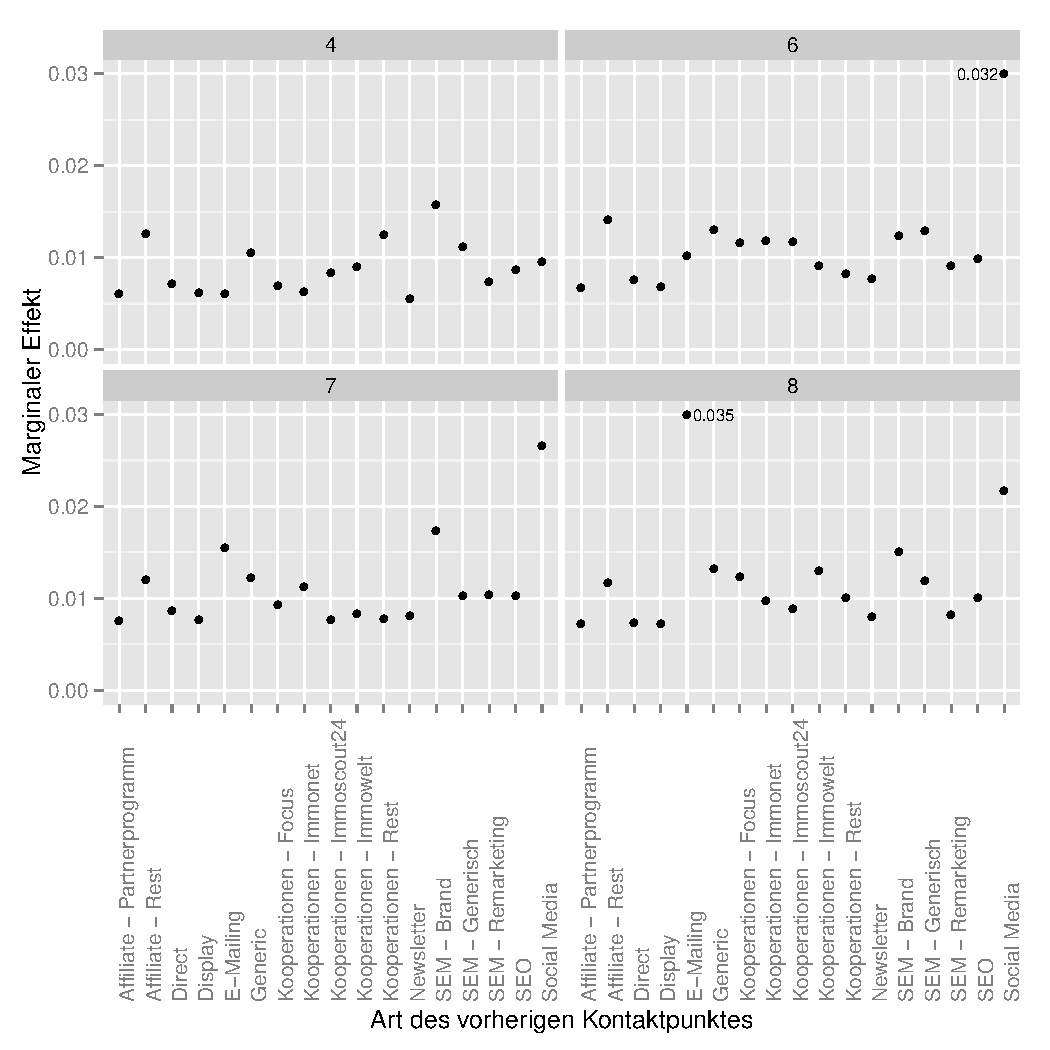
\includegraphics[scale=0.75]{marg_eff_campaignLast.pdf}\caption[Marginaler Effekt von \textit{CampaignLast}]{Marginaler Effekt des Features \textit{CampaignLast} an den Positionen $4$, $6$, $7$ und $8$}\label{marg_eff_campaignLast}
\end{figure}
\noindent An Position $2$ stechen neben \textit{Affiliate - Rest}, \textit{SEM - Brand} und \textit{E-Mailing} auch \textit{Direct} und \textit{Generic} durch ihre Marginalen Effekte leicht hervor. \textit{Direct} bedeutet, dass jemand im Browser direkt \textit{www.interhyp.de} eingegeben hat und \textit{Generic}, dass jemand über einen unbezahlten Link zur Interhyp kam.
Für die Positionen $3$ und $4$ ist vor allem \textit{Generic} wichtig. \textit{Display}, \textit{Social Media}, \textit{SEO} sowie die Kooperationen spielen, neben den bereits erwähnten, keine große Rolle für die ersten vier Positionen.\\
An den Positionen $4$, $6$ und $7$ ist \textit{CampaignLast} das zweitwichtigste Feature sowie an Position $8$ das wichtigste. Dessen marginalen Effekte sind in Abbildung \ref{marg_eff_campaignLast} dargestellt. Hier heben sich teilweise die selben Kategorien hervor, wobei die Unterschiede zwischen den Kampagnen kleiner sind. Überraschend ist, dass hier auch \textit{Social Media} einen starken Effekt hat. Allerdings liegen hierfür kaum Daten vor, wie in Abbildung \ref{campaign} zu erkennen ist.
\begin{figure}[H]
	\centering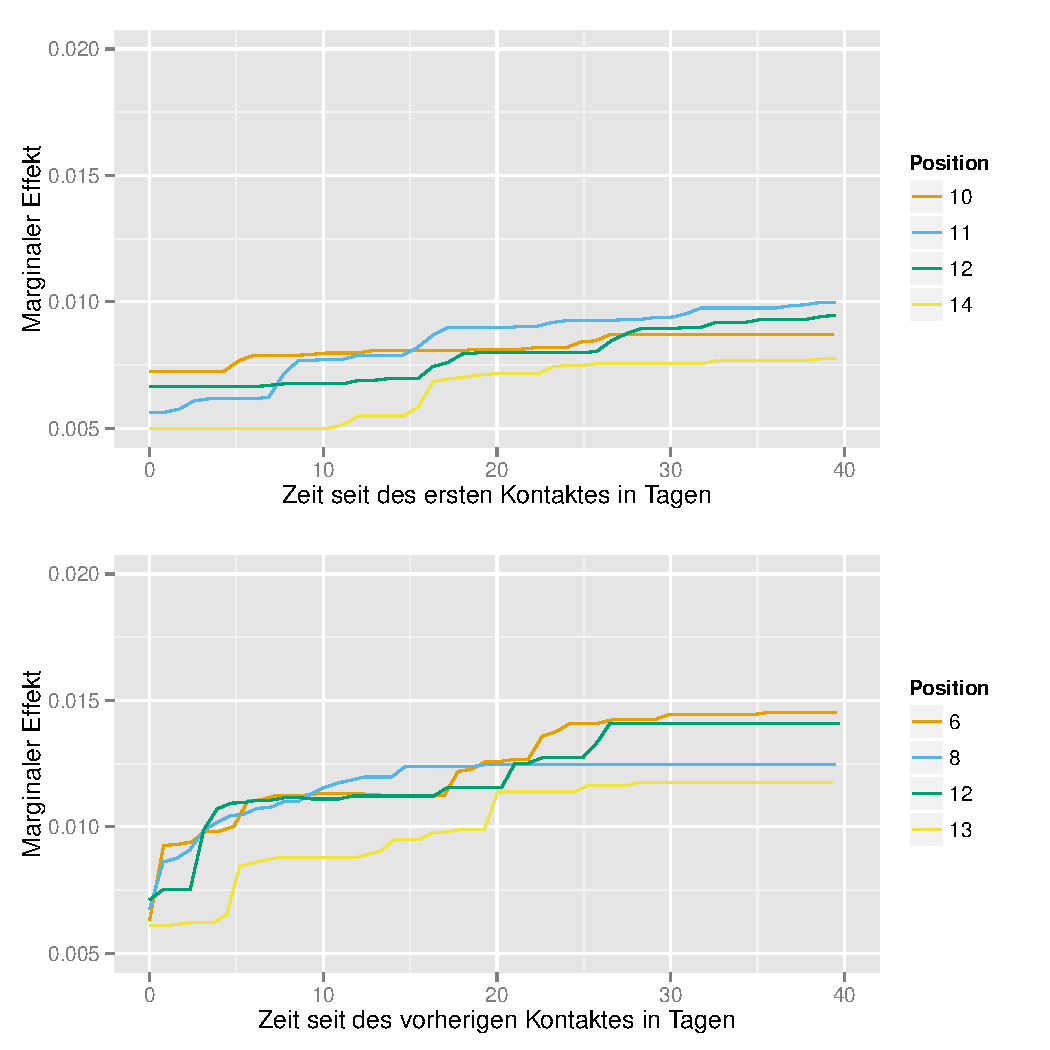
\includegraphics[scale=0.75]{marg_eff_time.pdf}\caption[Marginaler Effekt von \textit{TimeSinceFirst} und \textit{TimeSinceLast}]{Marginaler Effekt des Features \textit{TimeSinceFirst} an den Positionen $10$, $11$, $12$ und $14$ (oben) und des Features \textit{TimeSinceLast} an den Positionen $6$, $8$, $12$ und $13$ (unten)}\label{marg_eff_time}
\end{figure}
\noindent Das Feature \textit{TimeSinceFirst} ist an den Positionen $10$ und $14$ das wichtigste sowie an Position $11$ und $12$ das zweit- beziehungsweise drittwichtigste. \textit{TimeSinceLast} ist an den Positionen $6$, $12$ und $13$ das wichtigste Feature und an Position $8$ das zweitwichtigste Feature. Die marginalen Effekte für diese Positionen sind in Abbilung \ref{marg_eff_time} dargestellt, wobei diese an anderen Positionen ähnlich aussehen. Auf der $x$-Achse ist die Zeit in Tagen aufgetragen und auf der $y$-Achse die Marginalen Effekte. Für beide Features und alle Positionen steigen die marginalen Effekte mit der Zeit, wobei der Effekt bei \textit{TimeSinceLast} etwas größer ist.\\
Dass die Konvertierungswahrscheinlichkeit bei zeitlich längeren Funnels höher ist, könnte man dadurch erklären, dass die Entscheidung für den Bau eines Hauses oder ähnlichem und das damit verbundene Ausfüllen eines Online-Antrages viel Zeit in Anspruch nimmt. Dass für die Zeit seit des vorherigen Kontaktes der selbe Effekt auftritt, könnte man ähnlich erklären. Bei der Entscheidung für eine Baufinanzierung sind viele Dinge zu beachten. So erscheint es plausibel, dass sich interessierte Kunden eine längere Zeit auch offline mit dem Thema beschäftigen und später wieder online den Kontakt zur Interhyp AG suchen.\\
Bis hierhin wurden die Ergebnisse des, auf den Trainingsdaten geschätzten, Modells vorgestellt. Nun soll das Modell auf die Testdaten angewendet werden, um die Prognosegüte zu beurteilen.
\begin{figure}[H]
	\centering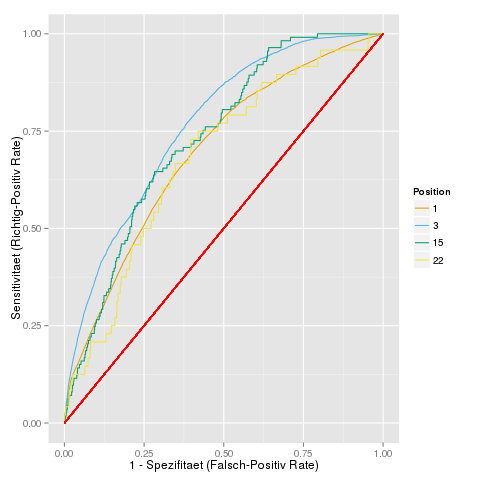
\includegraphics[scale=0.6]{roc.png}\caption[ROC-Kurve]{ROC-Kurve für die Positionen $1$, $3$, $15$ und $22$}\label{roc}
\end{figure}
\noindent Wenn man die geschätzte Prognosefunktion auf die Testdaten anwendet, bekommt man für jede Position und jede ID aus den Testdaten die Hazardrate, das heißt die Wahrscheinlichkeit an einer bestimmten Position zu konvertieren. Diese sind sowohl für konvertierte als auch nicht-konvertierte Funnels sehr niedrig, da die absolute Anzahl an nicht-konvertierten Funnels deutlich überwiegt. Um die Prognosegüte des Modells näher zu betrachten wurde deshalb für jede Position eine ROC-Kurve berechnet. Diese sind in Abbildung \ref{roc} für vier Positionen beispielhaft dargestellt.\\
Auf der $x$-Achse ist der Anteil der nicht-konvertierten Funnels, die als konvertiert vorhergesagt wurden aufgetragen und auf der $y$-Achse der Anteil der konvertierten Funnels, die auch als konvertiert vorhergesagt wurden. Je weiter die ROC-Kurve also oberhalb der roten Diagonalen liegt, desto besser kann das Modell zwischen konvertierten und nicht-konvertierten Funnels trennen. Für Position $3$ liegt die Kurve für alle Punkte überhalb der Kurve von Position $1$. Dies ist dadurch zu erklären, dass an Position $3$ mehr Informationen zur Erstellung des Modells verwendet werden als an Position $1$. Für Position $15$ und $22$ ist das Modell schlechter als an Position $3$. Die Kurven für die späteren Positionen sind deutlich rauher. Dies ist darauf zurück zu führen, dass dort weniger Datenpunkte vorhanden sind. Durch das Einbringen des Offsets kann die Prognoseleistung des Modells allerdings halbwegs konstant gehalten werden.\\
Dies ist in Abbildung \ref{auc} noch deutlicher zu erkennen. Hier ist die Fläche unterhalb der ROC-Kurve (AUC) für jede Position abgebildet. Dieser Wert fällt zwischen Position $15$ und $22$ unter $0.75$ ab, hält sich ansonsten aber relativ konstant auf $0.75$. Das heißt die Wahrscheinlichkeit, dass bei einer konvertierten Beobachtung die Hazardrate größer ist als bei einer nicht-konvertierten Beobachtung ist positionsübergreifend circa $0.75$.
\begin{figure}[H]
	\centering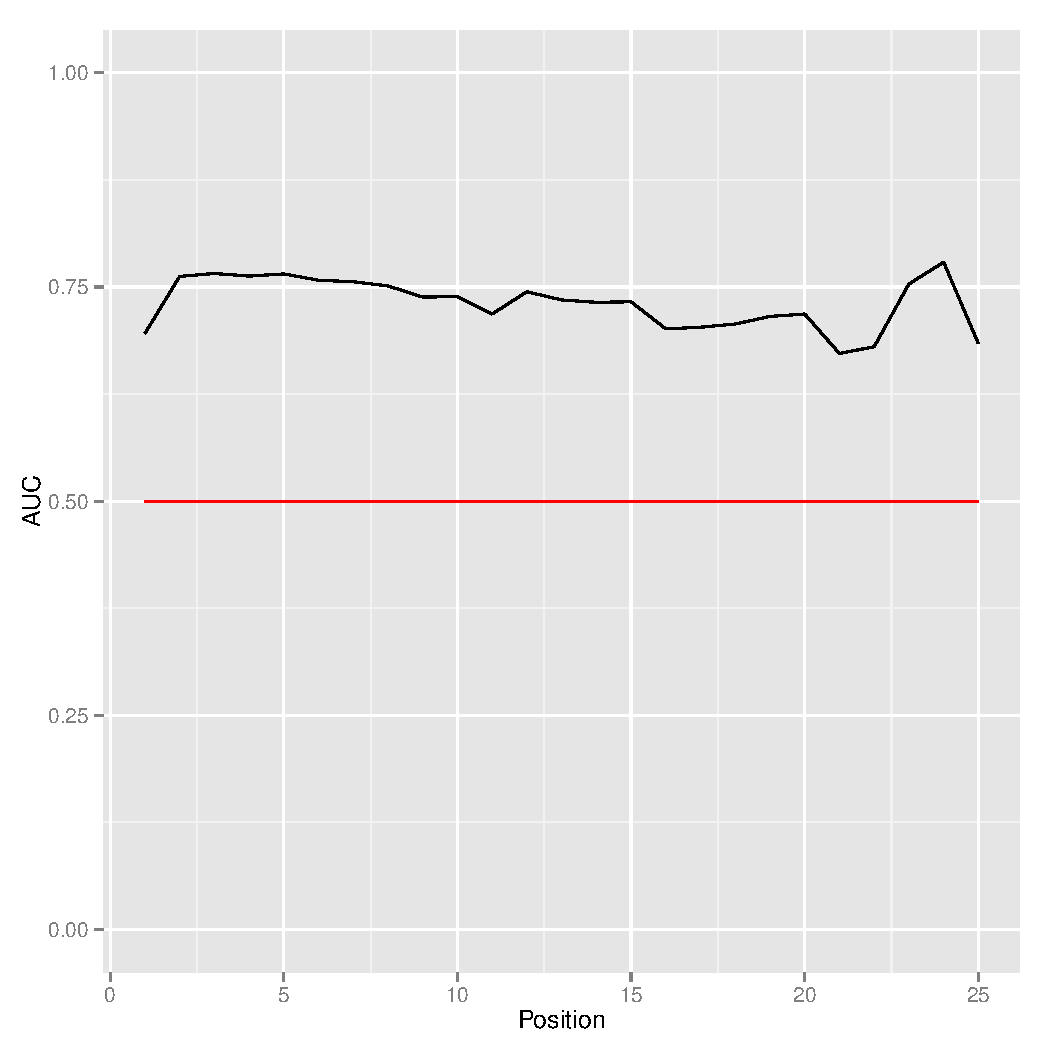
\includegraphics[scale=0.6]{auc.pdf}\caption[AUC-Wert]{AUC für alle Positionen}\label{auc}
\end{figure}

\subsection{Sequential Pattern Mining}\label{ergspm}

Der in Kapitel \ref{spm} beschriebene Algorithmus wurde zunächst seperat auf alle konvertierten sowie nicht-konvertierten Funnels angewendet. Dabei wurden Funnels mit der Länge eins ausgeschlossen, da in diesen offentsichtlich keine interessanten Sequenzen enthalten sein können. Der minimale Support wurde auf $0.05$ gesetzt, so dass nur Sequenzen, die in mindestens $5 \%$ aller Funnels vorkommen, als Ergebnis ausgegeben werden.
\begin{figure}[H]
	\centering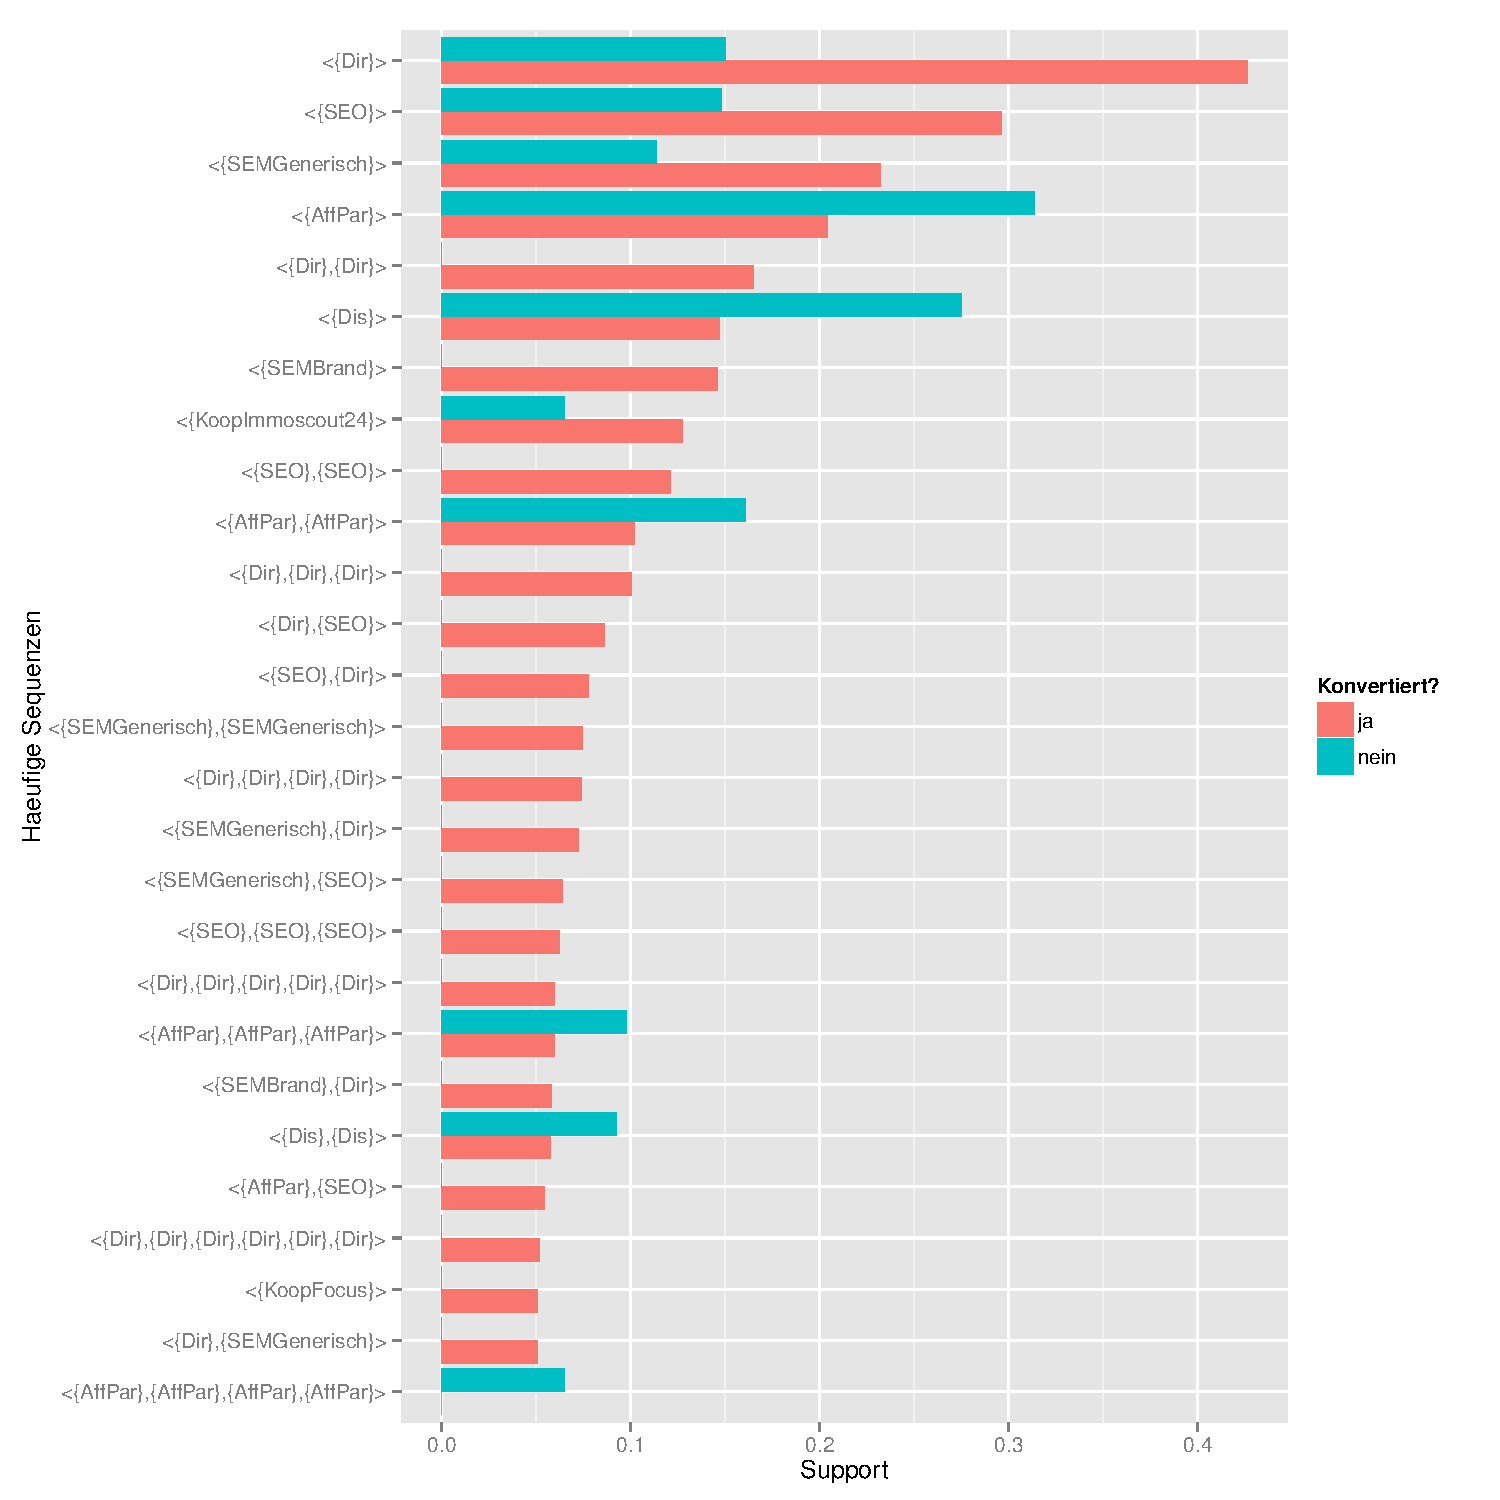
\includegraphics[scale=0.6]{spm_all.pdf}\caption[Häufige Sequenzen]{Häufige Sequenzen in den konvertierten und nicht-konvertierten Funnels}\label{spm_all}
\end{figure}
\noindent In Abbildung \ref{spm_all} sind diese Sequenzen geplottet, wobei auf der $x$-Achse der Suppport aufgetragen ist und die Sequenzen anhand des Supports der Sequenzen in den konvertierten Funnels absteigend geordnet sind. An den Stellen, wo keine Balken geplottet sind, war der Support kleiner als $0.05$. Die Namen der Kampagnen sind teilweise abgekürzt, um die Darstellung zu verbessern. \textit{AffPar} steht für \textit{Affiliate - Partnerprogramm}, \textit{Dir} für \textit{Direct} und \textit{Dis} für \textit{Display}. Außerdem ist zu beachten, dass die Sequenzen nicht exakt in der dargestellten Weise in den Funnels vorkommen müssen, sondern auch Abstände zwischen den aufeinanderfolgenden Kampagnen erlaubt sind.
\begin{figure}[H]
	\centering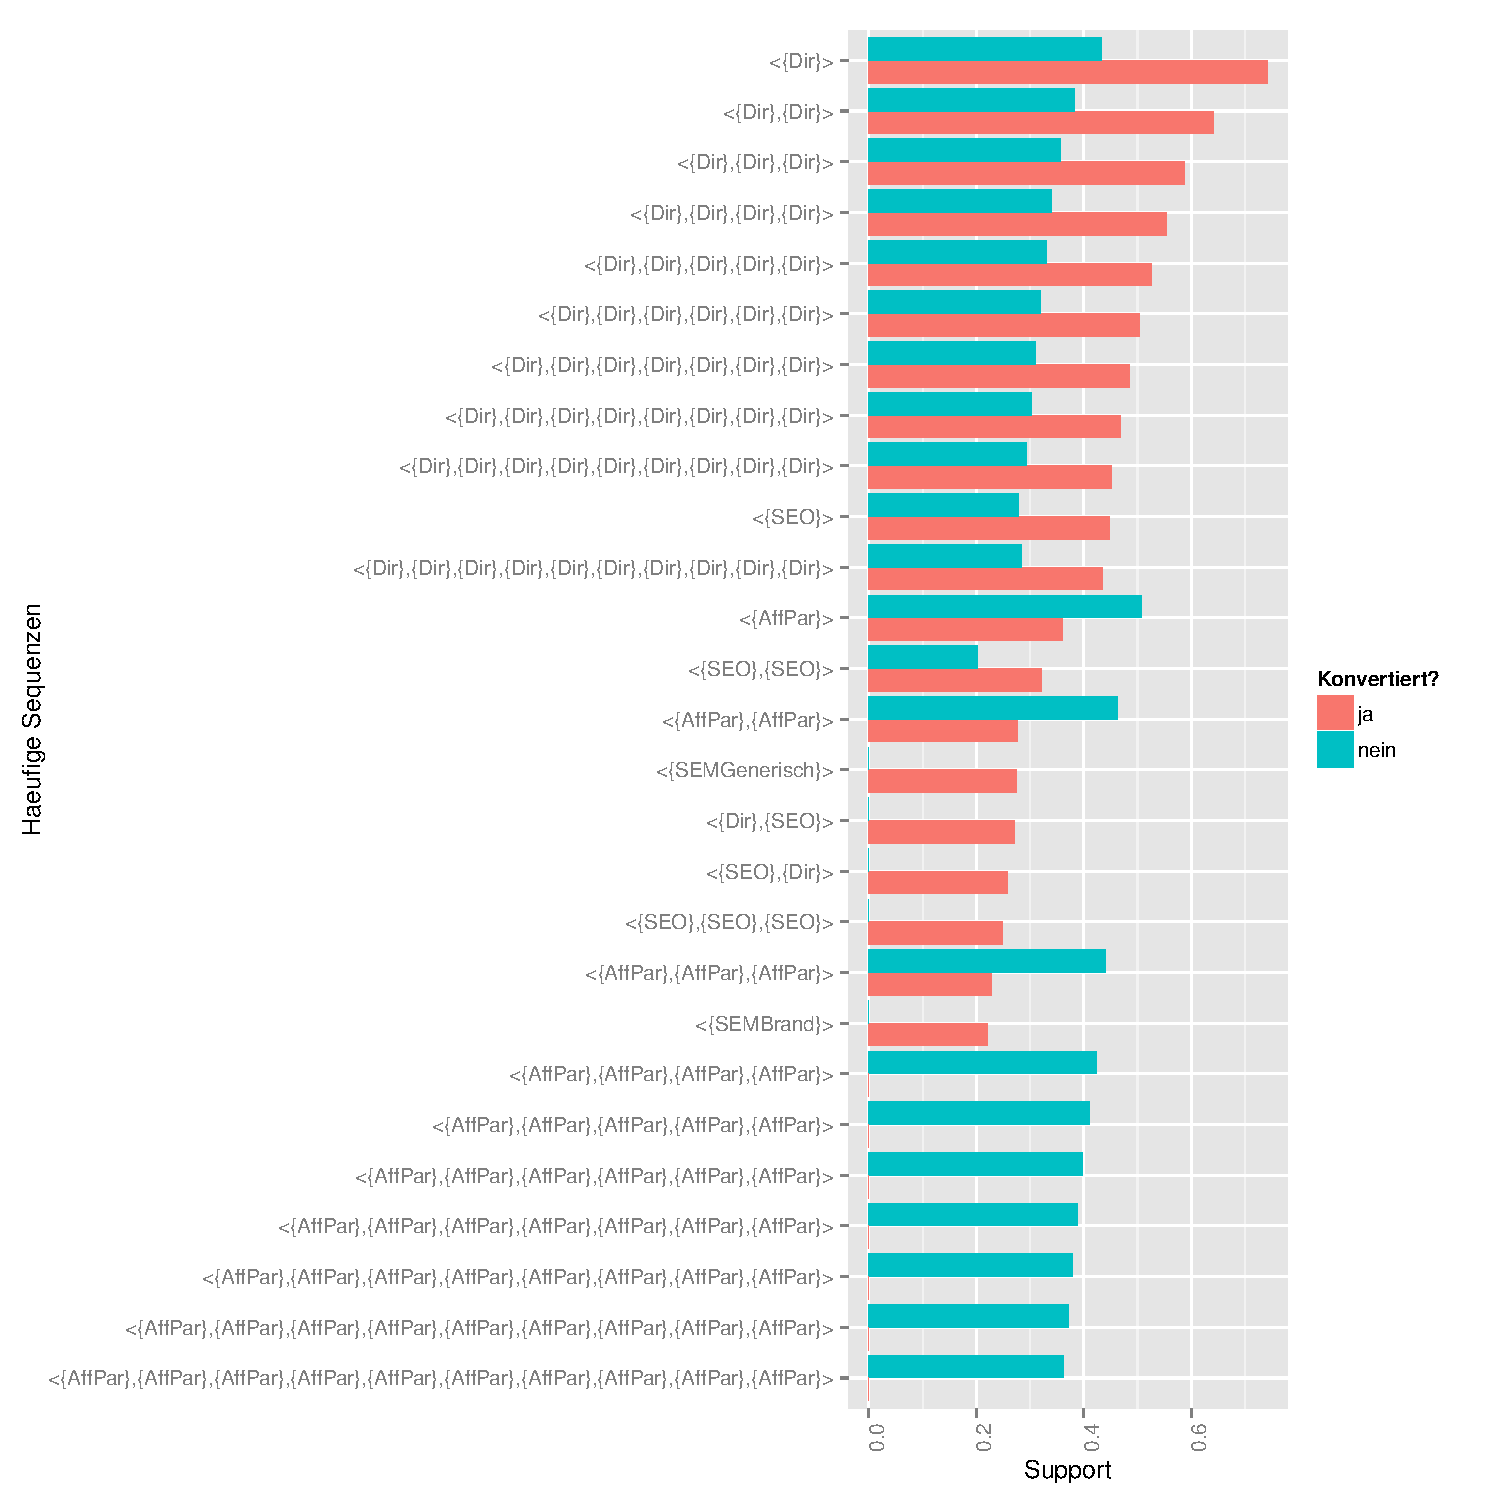
\includegraphics[scale=0.6]{spm_min15.pdf}\caption[Häufige Sequenzen in Funnels mit mindestens $15$ Kontaktpunkten]{Häufige Sequenzen in den konvertierten und nicht-konvertierten Funnels mit mindestens $15$ Kontakten}\label{spm_min15}
\end{figure}
\noindent Der Support von Sequenzen der Länge eins, wie \textit{<\{Dir\}>} oder \textit{<\{SEO\}>}, geben lediglich an, wie groß der Anteil der Funnels ist, die diese Kampagne mindestens einmal enthalten. Interessanter sind Sequenzen, die mindestens zwei Kampagnen enthalten. Hier fällt auf, dass Sequenzen mit wiederholtem \textit{Direct}-Kontakt in den konvertierten Funnels stärker sind. Umgekehrt sind  Sequenzen mit wiederholtem \textit{Affiliate - Partnerprogramm}-Kontakt in den nicht-konvertierten Funnels stärker. Allerdings haben die Sequenzen insgesamt einen sehr geringen Support. Das liegt vor allem daran, dass die Daten zu großem Teil aus sehr kurzen Funnels bestehen (siehe Abbildung \ref{funnelLength}).\\
Deshalb wurde der SPADE-Algorithmus erneut seperat auf konvertierte und nicht-konvertierte Funnel angewendet, wobei dieses mal nur Funnels verwendet wurden, die eine Mindestlänge von $15$ haben. Der minimale Support wurde auf $0.2$ erhöht, um die Anzahl an häufigen Sequenzen zu beschränken. Die Ergebnisse sind in Abbildung \ref{spm_min15} dargestellt.\\
Die Sequenzen haben jetzt teilweise einen Support, der größer als $0.5$ ist, das heißt mehr als die Hälfte der Funnels beinhalten diese Sequenz. Hier ist noch deutlicher zu erkennen, dass die \textit{Direct}-Sequenzen in den konvertierten Funnels stärker sind als in den nicht-konvertierten Funnels. Die \textit{Affiliate - Partnerprogramm}-Sequenzen haben in den nicht-konvertierten Funnels einen Support von ungefähr $40 \%$ und in den konvertierten Funnels einen Support von unter $20 \%$.\\

\subsection{Netzwerk}\label{resultsnetwork}

Mit dem Programm \textit{Gephi} ist es möglich interaktiv mit dem Netzwerk zu arbeiten. Eine komplette Analyse des Netzwerkes würde den Rahmen dieses Berichtes sprengen. Deshalb soll hier nur beispielhaft, anhand einiger Grafiken, dargestellt werden, welche Ergebnisse man aus dem Netzwerk ziehen kann. Dafür wurde ein Ausschnitt an Position $2$ gewählt. Eine genauere Anleitung zur Verwendung von \textit{Gephi} ist zudem in Kapitel \ref{anhang} zu finden.

\subsubsection*{Relative Ausgänge}

Zunächst werden die relativen Ausgänge präsentiert, das heißt die Gewichte aller Kanten, die einen Knoten verlassen, ergeben in der Summe $1$.\\
Abbildung \ref{out_labels} enthält den Ausschnitt des Netzwerkes an Position $2$ mit den relativen Ausgängen. Die Knoten sind farblich codiert und mit Labels versehen. Am rechten Bildrand ist noch eine Kampagne der ersten Position \textit{SEO\_1} zu erkennen. Von dort und den anderen Kampagnen der ersten Position führen die Kanten zu den Kampagnen der zweiten Position in der Mitte der Abbildung. Für Funnels, die mehr als zwei Kontaktpunkte haben gehen die Kanten von diesen Kampagnen zu den Knoten der dritten Positionen jenseits des linken Bildrandes. Die Kampagne \textit{Affiliate - Partnerprogramm\_3} ist noch zu erkennen.\\
Funnels, die lediglich über zwei Kontaktpunkte verfügen, enden in \textit{Fail\_2} im Falle einer Nicht-Konvertierung beziehungsweise in \textit{Success\_2} im Falle einer Konvertierung.
\begin{figure}[H]
	\centering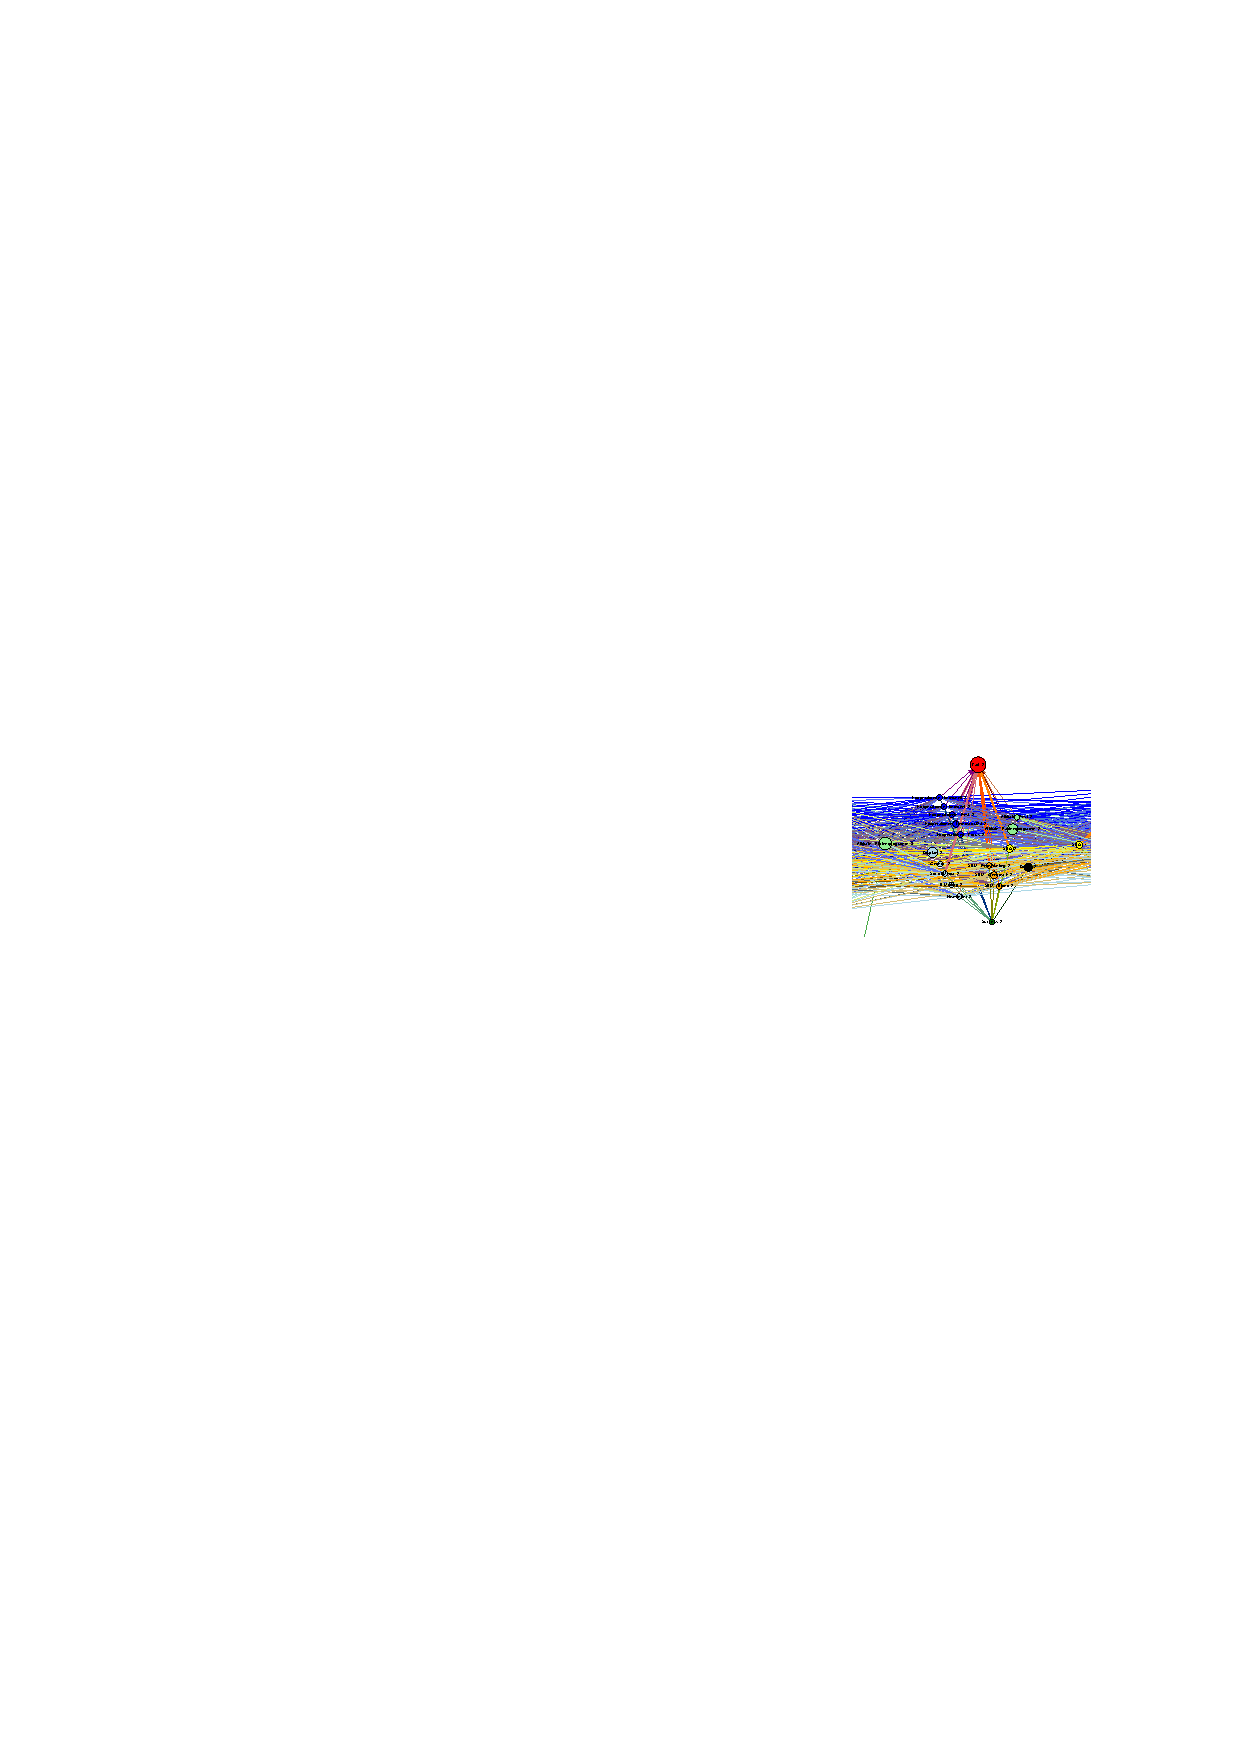
\includegraphics[scale=2.3]{out_labels.pdf}\caption[Relative Ausgänge]{Auschnitt des Netzwerkes an Position $2$ mit relativen Ausgängen}\label{out_labels}
\end{figure}
Die Dicke der Kanten hängt von deren Gewichtung ab. Abbildung \ref{out_filter_2_succ} enthält den selben Ausschnitt, wobei nun ein Filter von $0.02$ auf die Kanten angewendet wurde. Somit sind nur noch Kanten abgebildet, deren Gewicht größer als $0.02$ ist. Durch das Auswählen des Knoten \textit{Success\_2} werden alle Knoten hervorgehoben, die nach der Anwendung des Filters noch durch eine Kante mit \textit{Success\_2} verbunden sind.
\begin{figure}[H]
	\centering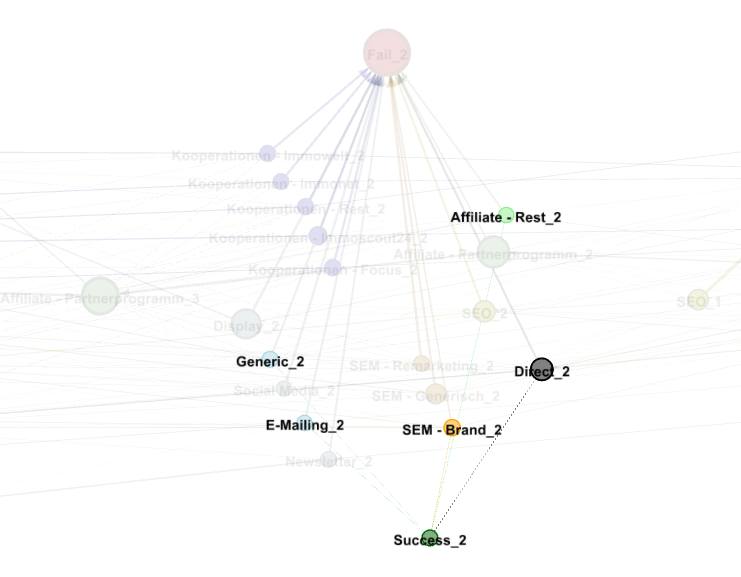
\includegraphics[scale=0.35]{out_filter_2_succ.png}\caption[Relative Ausgänge mit Filter $0.02$]{Auschnitt des Netzwerkes an Position $2$ mit relativen Ausgängen, Filter $0.02$ und Fokus auf den konvertierten Funnels}\label{out_filter_2_succ}
\end{figure}
Das heißt über $2 \%$ aller Nutzer, die als zweiten Kontaktpunkt $Direct$ haben, konvertieren an der zweiten Position. Selbiges gilt für \textit{Affiliate - Rest}, \textit{Generic}, \textit{SEM - Brand} und \textit{E-Mailing}. Durch Veränderung der Filter und weiterer Einstellungen können die Ergebnisse auch noch genauer betrachtet werden. Wie bereits erwähnt, ist in Kapitel \ref{anhang} ein Tutorial dazu vorhanden.\\
Interessant ist an dieser Stelle, dass die fünf hervorgehobenen Kampagnen gleichzeitig die fünf stärksten Kampagnen bei den Marginalen Effekten des Features \textit{Campaign} an Position $2$ sind. Das heißt die Ergebnisse des Survival-Modells können durch die Betrachtung des Netzwerkes überprüft und bestätigt werden.\\
Abbildung \ref{out_filter_50_fail} enthält erneut den selben Ausschnitt des Netzwerkes, wobei nun ein Filter von $0.5$ angewendet wurde und der Fokus auf den nicht-konvertierten Funnels liegt. Von den hervorgehobenen Knoten enden also jeweils mindestens die Hälfte der Beobachtungen ohne Konvertierung.\\
Analog zu der Betrachtung von \textit{Success\_2} oder \textit{Fail\_2} können auch die Kampagnen durch Auswählen näher betrachtet werden. Durch die positionsübergreifende Betrachtung können zudem die häufigen Sequenzen, die mittels des Sequential-Pattern-Mining Algorithmus ermittelt wurden, erkannt werden.
\begin{figure}[H]
	\centering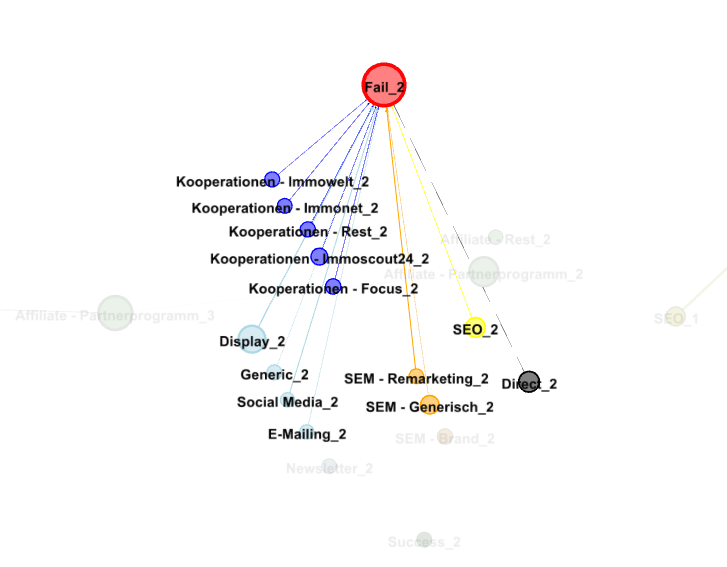
\includegraphics[scale=0.35]{out_filter_50_fail.png}\caption[Relative Ausgänge mit Filter $0.5$]{Auschnitt des Netzwerkes an Position $2$ mit relativen Ausgängen, Filter $0.5$ und Fokus auf den nicht-konvertierten Funnels}\label{out_filter_50_fail}
\end{figure}

\subsubsection*{Relative Eingänge}

In diesem Abschnitt wird erneut Position $2$ betrachtet, wobei die Kanten nun anhand der relativen Eingänge gewichtet sind. Das heißt die Gewichte aller Kanten, die in einen bestimmten Knoten gehen, ergeben aufsummiert $1$. Abbildung \ref{in_labels} enthält den Ausschnitt des Netzwerkes. Am rechten beziehungsweise linken Bildrand ist erneut eine Kampagne von Position $1$ beziehungsweise $3$ zu erkennen. Die Farben und Beschriftungen der Knoten sind die selben wie in Abbildung \ref{out_labels}. 
\begin{figure}[H]
	\centering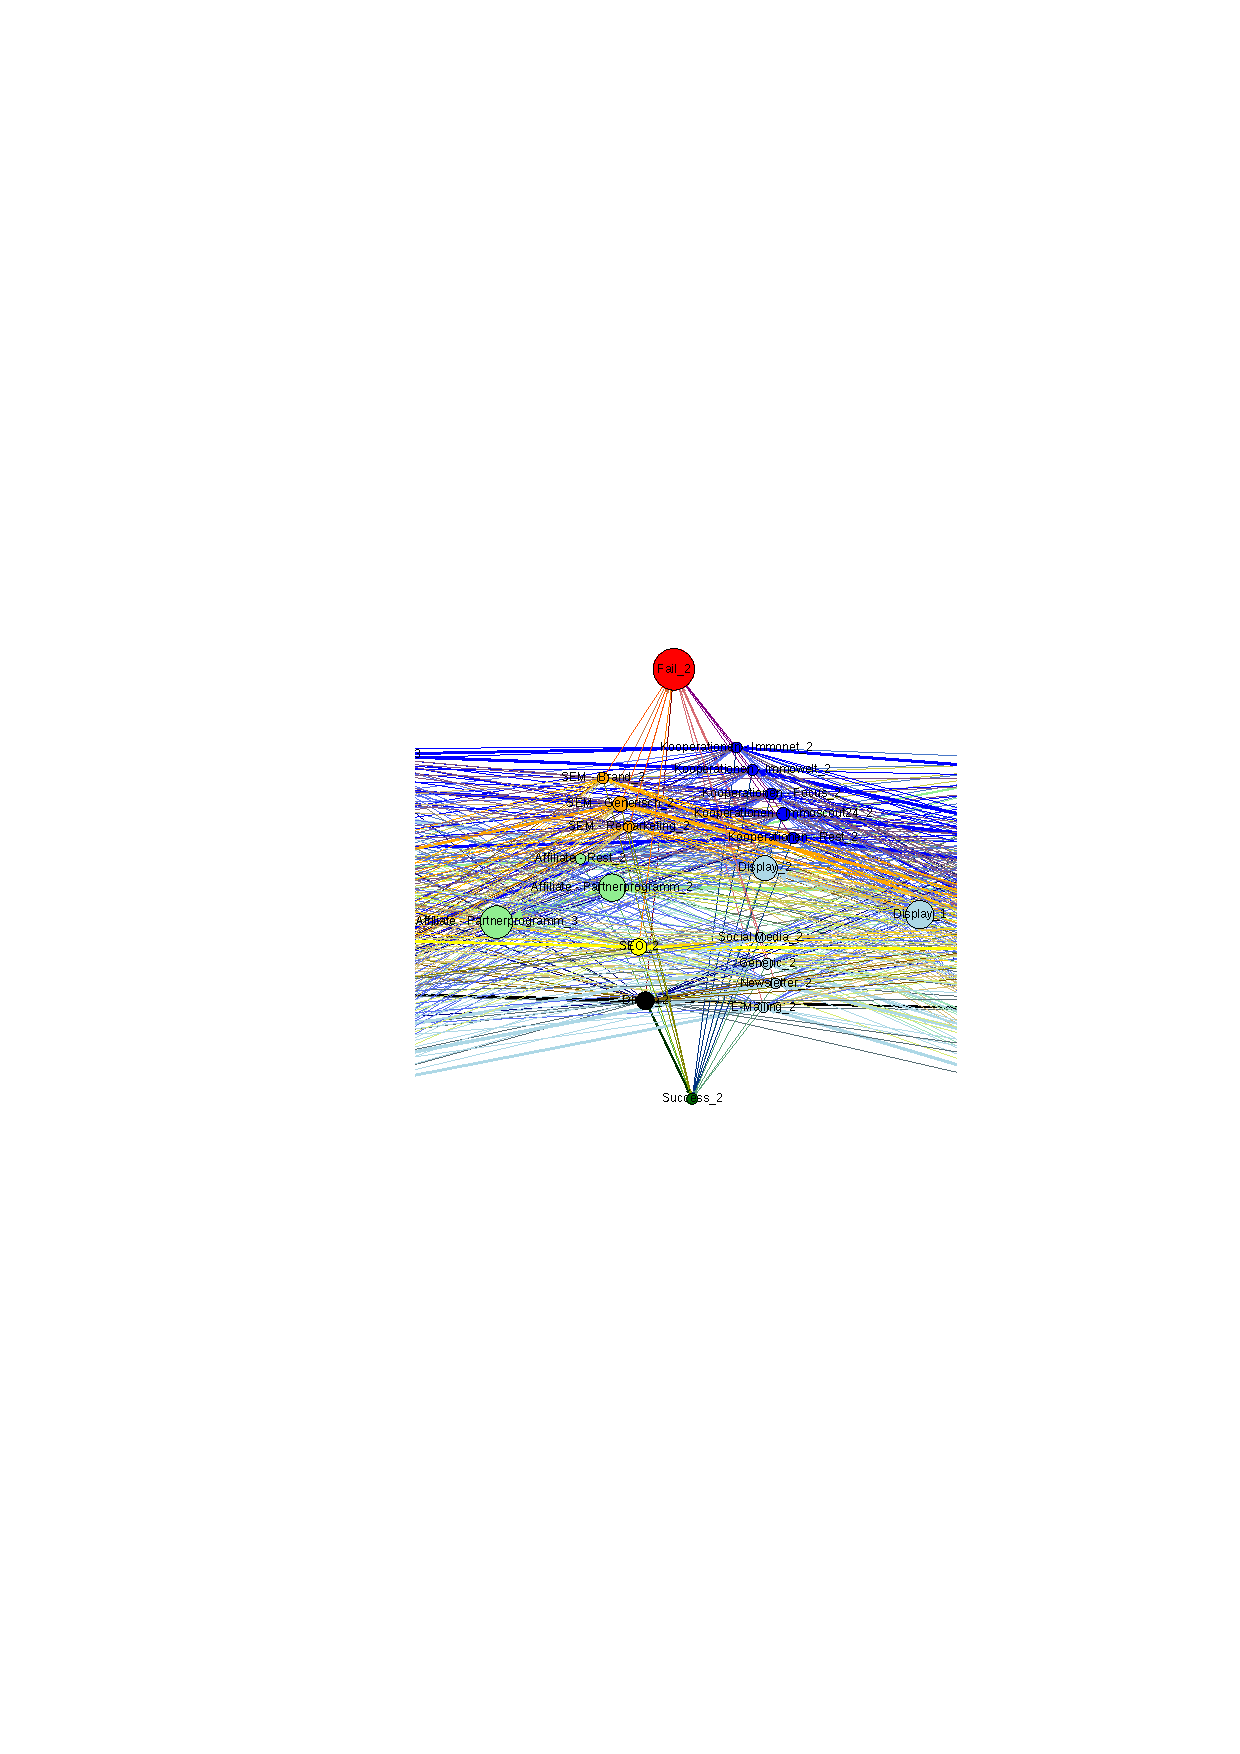
\includegraphics[scale=0.9]{in_labels.pdf}\caption[Relative Eingänge]{Auschnitt des Netzwerkes an Position $2$ mit relativen Eingängen}\label{in_labels}
\end{figure}
\noindent Auf diesen Ausschnitt wurde ein Filter von $0.1$ angewendet, wobei der Fokus auf den konvertierten Funnels liegt. Der resultierende Graphh ist in Abbildung \ref{in_filter_10_succ} zu sehen.
\begin{figure}[H]
	\centering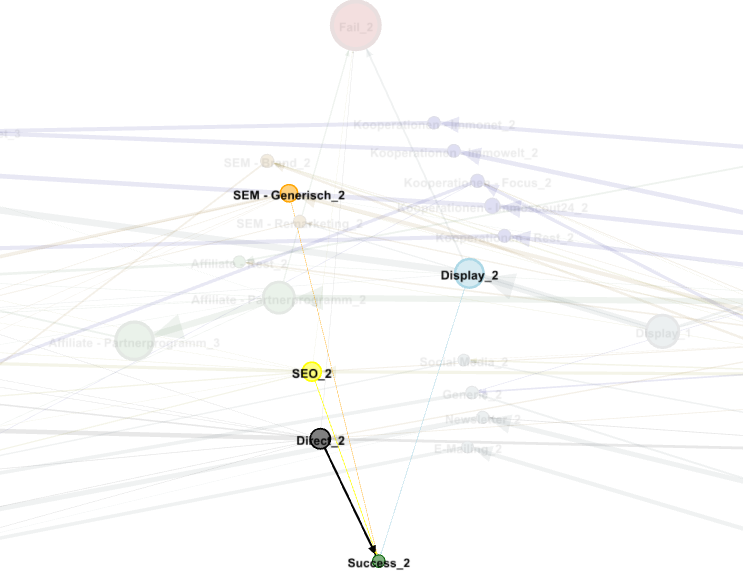
\includegraphics[scale=0.35]{in_filter_10_succ.png}\caption[Relative Eingänge mit Filter $0.1$ und Fokus auf Konvertierten]{Auschnitt des Netzwerkes an Position $2$ mit relativen Eingängen, Filter $0.1$ und Fokus auf den konvertierten Funnels}\label{in_filter_10_succ}
\end{figure}
\noindent Die hervorgehobenen Knoten \textit{SEM-Generisch\_2}, \textit{Display\_2}, \textit{SEO\_2} und \textit{Direct\_2} machen jeweils mehr als $10 \%$ der konvertierten Funnels aus, die aus zwei Kontaktpunkten bestehen. Das heißt hier kann nun betrachtet werden, aus welchen Kampagnen des letzten Kontaktpunktes sich die Menge der konvertierten beziehungsweise nicht-konvertierten Funnels zusammensetzen. Zudem ist es auch möglich eine Kampagne zu markieren, so dass erkennbar wird, aus welchen Kampagnen der vorherigen Position, sich diese zusammensetzt. Im Gegensatz dazu, war die Interpretation im vorherigen Kapitel eine andere. Dort wurde betrachtet, wohin die Nutzer von einem Knoten aus gehen.\\
Abbildung \ref{in_filter_10_fail} enthält den selben Ausschnitt mit dem selben Filter von $0.1$, wobei nun die nicht-konvertierten Funnels betrachtet werden. Das heißt von den Funnels, die nach zwei Kontaktpunkten ohne Konvertierung abbrechen, haben jeweils mindestens $10\%$ als letzten Kontaktpunkt \textit{Affiliate - Partnerprogramm\_2}, \textit{Display\_2}, \textit{SEO\_2} oder \textit{Direct\_2}.
\begin{figure}[H]
	\centering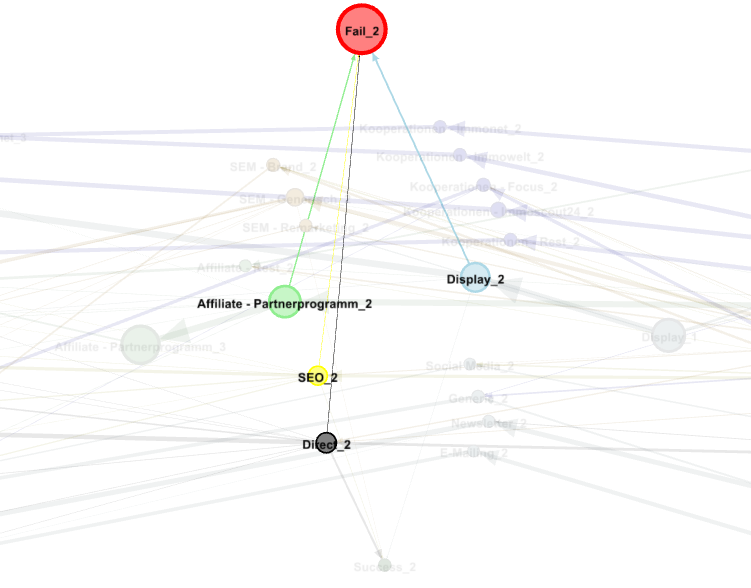
\includegraphics[scale=0.35]{in_filter_10_fail.png}\caption[Relative Eingänge mit Filter $0.1$ und Fokus auf Nicht-Konvertierten]{Auschnitt des Netzwerkes an Position $2$ mit relativen Eingängen, Filter $0.1$ und Fokus auf den nicht-konvertierten Funnels}\label{in_filter_10_fail}
\end{figure}
\section{Zusammenfassung}\label{zusammenfassung}

An dieser Stelle sollen die angewendeten Methoden und Ergebnisse noch einmal kurz zusammengefasst werden.\\
Es wurde ein zeitdiskretes Survival-Modell aufgestellt, dass für jede Beobachtung an jeder Position die Konvertierungswahrscheinlichkeit schätzt. Dieses Modell kann als Klassifikator in konvertierte und nicht-konvertierte Funnels fungieren. Die Prognosegüte konnte vor allem durch die Anwendung von Stochastic Gradient Boosting und die Einführung des Offsets verbessert werden. Außerdem liefern die Marginalen Effekte der Features eine gute Interpretationsmöglichkeit der Prädiktorfunktion.\\
Die wichtigsten Ergebnisse an dieser Stelle sind, dass die Kampagnen \textit{Affiliate - Rest}, \textit{E-Mailing}, \textit{SEM - Brand}, \textit{Direct} und \textit{Generic} im Vergleich zu den restlichen Kampagnen besonders gut für die Konvertierung funktionieren. Außerdem haben Funnels mit einer längeren Beobachtungsspanne und einer niedrigeren Frequenz von Kontaktpunkten eine höhere Konvertierungswahrscheinlichkeit.\\
Die Einführung von Interaktionen in das Modell hat zu einer Verschlechterung der Prognoseleistung geführt und wurde deshalb nicht weiter verfolgt. Außerdem konnten die \textit{Views} aufgrund der Datenlage in den statistischen Analysen nicht berücksichtigt werden.\\
Mit dem Sequential Pattern Mining-Algorithmus sollten häufige Sequenzen in den Funnels entdeckt werden. Von den resultierenden Ergebnissen sind die \textit{Direct}-Sequenzen in den konvertierten und die \textit{Affiliate - Partnerprogramm}-Sequenzen in den nicht konvertierten Funnels erwähnenswert. Allerdings ist zu berücksichtigen, dass zwischen den einzelnen Elementen der Sequenzen auch andere Kampagnen erlaubt sind. Ein weiterer Ansatz wäre nur diejenigen Funnels zu berücksichtigen, die die Sequenzen in der exakten Reihenfolge ohne Lücken vorweisen. Bei der gegebenen Datenlage würde das allerdings zu einer drastischen Reduzierung des Supports der Sequenzen führen, zumal der Support der häufigen Sequenzen aufgrund der überwiegenden Anzahl an kurzen Funnels ohnehin nicht sehr groß ist. Um interessantere Ergebnisse zu erlangen, wurden die Daten deshalb noch in Form eines Netzwerkes visualisiert.\\
Dieses Netzwerk erlaubt die Visualisierung der gesamten Daten. Außerdem können durch die Gewichtung der Kanten mit den relativen Ein- und Ausgängen wertvolle Informationen aus den Daten gezogen werden. Mit Hilfe des, in diesem Bericht bereitgestellten, Tutorials (siehe Kapitel \ref{anhang}) ist ein interaktives Arbeiten mit dem Netzwerk sowie eine weiterführende Erforschung der Daten möglich.

\begin{frame}
	\centering \huge
	Vielen Dank für Ihre Aufmerksamkeit!
\end{frame}

\end{document}

